\documentclass[12pt]{third-rep}

%% Any characters from a % to the end of line are comments.

%% The third-rep class and this starter kit were written by 
%% Graham Gough <graham@cs.man.ac.uk>
%% If you have any comments or questions regarding this document,
%% please post them to the local newsgroup man.cs.tex.

%% This skeleton report is organised as a master file called
%% report.tex which then includes files for individual parts including
%% abstract.tex, chapter1.tex, chapter2.tex, chapter3.tex and
%% appendix1.tex.  

%% The third-rep style is a locally created style based on the
%% standard LaTeX report style. If you really want to have a look at
%% it, its source can be found in
%% /usr/local/share/texmf/tex/latex/mancs/third-rep.cls
%%
%% More information about LaTeX in general and the local setup in
%% particular can be found on the web at 
%% http://csis.cs.manchester.ac.uk/software/contrib/latex
%%
%%%%%%%%%%%%%%%%%%%%%%%%%%%%%%%%%%%%%%%%%%%%%%%%%%%%%%%%%%%%%%%%%%%%%%%%
%%
%% This is an example of how you load extra packages.
%% Some packages are already loaded in the third-rep class

\usepackage{url} % typeset URL's sensibly

\usepackage{pslatex} % Use Postscript fonts

%% The best way to latex just one chapter is to uncomment lines such as
%% the next:
%\includeonly{chapter1}

%% This defines the title (the \\ forces a line break)
\title{Image-to-Image Translation\\
  Using Generative Adversarial Networks}
%% and author
\author{Wenchang Liu}
%% and supervisor
\supervisor{Prof. Angelo Cangelosi}
%% and the year of the report
\reportyear{2020}

%% this defines the file that contains the text of the abstract, there
%% must be one of these by the time you submit your report.
\abstractfile{abstract.tex}

%% this defines the file that contains the acknowledgements (it can be
%% omitted if you don't feel like thanking anyone
\thanksfile{merci.tex}

%% Uncomment the following lines if you want to include the date as a
%% header in draft versions. See the documentation for fancyhdr for
%% more ways of modifying headers (texdoc fancyhdr will show you the
%% docs) 

%\usepackage{fancyhdr}
%\pagestyle{fancy}
%\lhead{}  % left head
%\chead{Draft: \today} % centre head
%\lfoot{}
%\cfoot{\thepage}
%\rfoot{}

%% The following line sets up the use of PostScript fonts rather
%% than the standard bitmapped fonts.
\usepackage{pslatex}

%% Uncomment the following line if you want to change the name of the
%% Bibliography to References
%\renewcommand{\bibname}{References}

\usepackage{listings}
\usepackage{parskip}
\usepackage[namelimits]{amsmath} %数学公式
\usepackage{amssymb}             %数学公式
\usepackage{amsfonts}            %数学字体
\usepackage{mathrsfs}            %数学花体
\usepackage{float}
\usepackage[colorlinks, linkcolor=black]{hyperref}
\usepackage{booktabs}
\usepackage{longtable}

%% End of preamble, the actual document starts here
%%

\begin{document}

%% This actually creates the title and abstract pages
\dotitleandabstract

%% Generate contents etc
\tableofcontents
\listoffigures
\listoftables

\hypersetup{
  linkcolor=red
}

%% These include the actual text
\chapter{Introduction and Background}
\label{cha:intro}
This chapter briefly introduces the problem of image-to-image translation,
deep learning and Generative Adversarial Networks. General ideas of these topics
are very useful for the reader to grasp the more complicated concepts that 
the report talking about in the later chapters.

\section{Image-to-Image Translation}
\subsection{Definition}
Many challenges in computer vision and machine learning can be regarded as “translating” an 
input image into a corresponding output image. As we all know that a concept may be expressed in either 
English or Chinese, a scene can be represented as various forms including RGB images, gradient fields, 
edge maps, segmentation maps, etc. Similar to machine translation of languages, we cite the definition
of image translation from Isola et al.: “tasks of automatically translating
one possible representation of a scene into another”\cite{pix2pix2016}. Researchers have solved some kinds of image 
translation using independent, specific-purpose machinery(e.g. style transfer\cite{gatys2015neural}),
even if the settings of these problems are the same: predict pixels from pixels.
The models this report discuss (originated from \cite{pix2pix2016})
make using one common framework for all these problems possible.
In this project, we will focus on translating 
semantic segmentation maps into photorealistic images but you can apply these approaches on
other types of image translation problems.

\subsection{Segmentation Maps}
In computer vision, image segmentation is often needed in order to switch to 
different representations of an image especially to those representations that 
are more meaningful and simpler for analysis\cite{wikipedia},
and a lot of deep learning algorithms have been invented to do semantic labeling. Therefore,
the data this project needs is easy to acquire.

Segmentation maps are also known as semantic label maps, which is a set of segments 
that collectively cover the entire image\cite{wikipedia}. Each region contains similar pixels 
in terms of the semantic of the image and each region is assigned with a different 
color and a semantic label.

The following figure \ref{fig:segmentation-map-example} is an example segmentation map image, where each color represent one type of object:
\begin{figure}[H]
    \begin{center}
    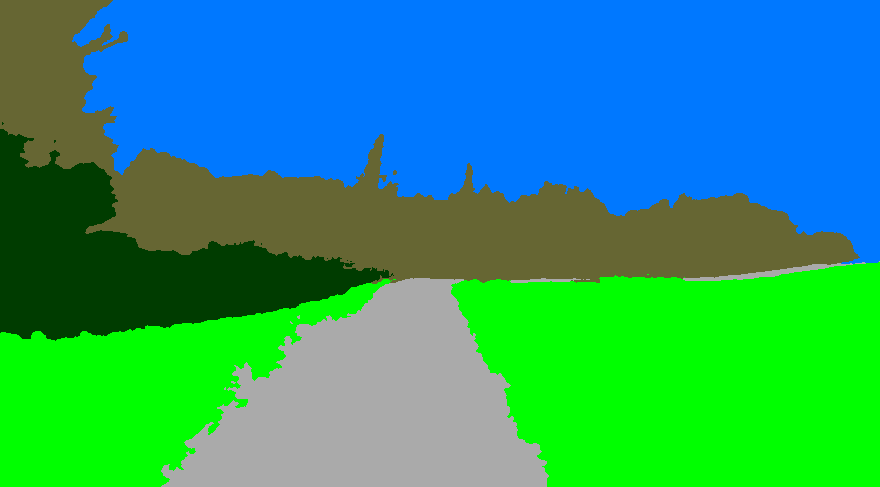
\includegraphics[width=8cm]{figures/seg-map-eg}
    \end{center}
    \caption{A Segmentation Map}
    \label{fig:segmentation-map-example}
\end{figure}

\subsection{Applications}
The translation of photorealistic images from sketches will be very useful once this technology
is mature enough for commercial uses. Designers could get a fast preview of 
their work not by imagination, but with vivid photorealistic images. For example, 
game designers can preview the scene, items, or characters they design vividly by drawing 
just sets of color blocks or edges. Besides, this technology provides opportunities for 
people who are not good at art to create their own masterpieces.


\section{Deep Learning}
\nocite{articleDL}
\nocite{Goodfellow-et-al-2016}
Deep learning is a member of the machine learning algorithms family, based on
artificial neural networks and representation learning\cite{wikipedia}(i.e. automatically discover 
representations needed for feature detection or classification from raw data). 
Learning can be supervised, semi-supervised, or unsupervised. Deep learning approaches have widely
been applied to fields including computer vision(CV), natural language processing(NLP), 
reinforcement learning(RL), text filtering, machine translation, image synthesis, drug design, etc., 
where they perform comparably to and in some cases better than human experts.  

\subsection{Neural Networks}
Artificial neural networks(ANN) are computing systems vaguely inspired by 
the biological neural networks that constitute animal brains\cite{wikipedia}. Neural networks used in deep learning 
can be regarded as a parametric approximation function that can map the input A into the output
B with parameters $\omega$ i.e. $f_{\boldsymbol{\omega}}: A \rightarrow B$. The mapping 
function can gradually get optimized by updating its parameters through raw data and 
back propagation algorithms. 

The multi-layer architecture of neural networks can achieve complex mappings by composing 
multiple but simple non-linear functions together.
In neural network implementations, the input “signal” will pass into each neuron(or node) through
connection edges, the output of each neuron is computed by some non-linear function of 
the sum of its inputs, typically, neurons are aggregated into layers and the “signals”
travel from the first input layer to the last output layer to produce the final results.
\begin{figure}[H]
    \begin{center}
    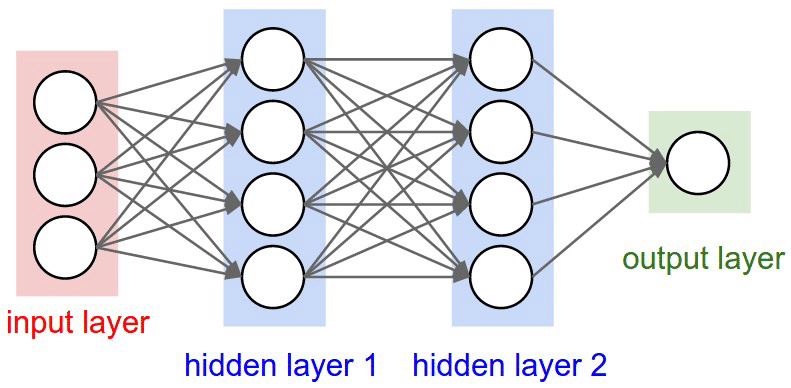
\includegraphics[width=8cm]{figures/nn-structure}
    \end{center}
    \caption{Neural Network Structure}
    \label{fig:neural-network-structure}
\end{figure}

\subsection{Activation Functions}
The activation function of a node(i.e. neuron) in neural networks determines the output of that node 
given an input or set of inputs. Note that only non-linear activation functions allow such networks 
to compute complex mappings, if we do not use activation function or use linear activation function,
no matter how many layers we have, we can only result in getting linear mapping functions.

The activation functions this project uses are the following(explanations referenced from \cite{cs231n}):
\begin{itemize}
    \item Rectified Linear Unit(ReLU)
    
    The Rectified Linear Unit is one of the simplest and most commonly used activation functions 
    in the last few years, it computes the function: $f(x)=\max(0,x)$. 
    This activation function is just threshold at zero, which is much simpler than tanh or sigmoid, 
    and it was found to greatly accelerate the convergence of gradient descent compared to other 
    activation functions including tanh or sigmoid. However, it does has a disadvantage of being fragile
    during training, i.e. the ReLU units can irreversibly die and forever be zero during training since 
    they can get knocked off the data manifold. 
    \begin{figure}[H]
        \begin{center}
        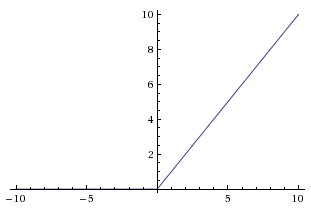
\includegraphics[width=5cm]{figures/relu}
        \end{center}
        \caption{Rectified Linear Unit(ReLU) Activation Function}
        \label{fig:ReLU}
    \end{figure}
    \item Leaky Rectified Linear Unit(Leaky ReLU)
    
    Leaky ReLUs are one type of approach trying to fix the "dying ReLU" problem. Instead of just threshold 
    at zero, it computes: $f(x)=1(x<0)(\alpha x)+1(x>=0)(x)$, where $\alpha$ is a small constant. Some report 
    leaky ReLUs are effective but the reuslts are necessarily consistent.
    \begin{figure}[H]
        \begin{center}
        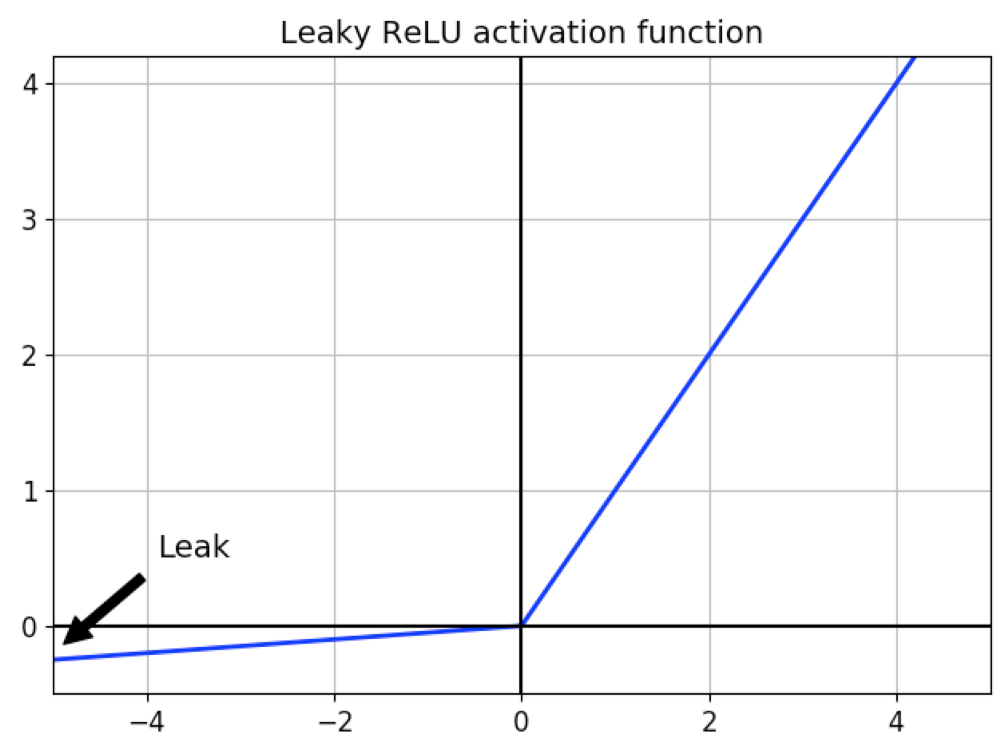
\includegraphics[width=5cm]{figures/leakyrelu}
        \end{center}
        \caption{Leaky ReLU Activation Function}
        \label{fig:Leaky ReLU}
    \end{figure}
    \item Hyperbolic Tangent(tanh)
    
    The tanh activation function squashes a real-valued number to the range of [-1, 1], this activation
    saturates but is zero-centered so that it can be regarded as a scaled and more desirable sigmoid 
    activation function in practice.
    \begin{figure}[H]
        \begin{center}
        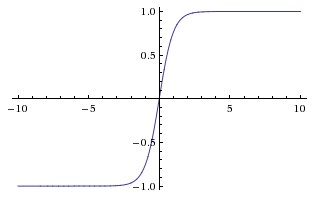
\includegraphics[width=5cm]{figures/tanh}
        \end{center}
        \caption{Hyperbolic Tangent Activation Function}
        \label{fig:tanh}
    \end{figure}
    
\end{itemize}

\subsection{Backpropagation}
Backpropagation(BP) is a widely used algorithm for neural networks training and
supervised learning. While training a neural network, there will be a loss function
$L$ describing how well the current approximation $f_{\boldsymbol{\omega}}$ approximates
the correct mapping function by calculate the differences between the output from the 
neural network and the ground-truth from a training dataset. Then the backpropagation algorithm 
will try to approximate the correct mapping function by continuing minimizing the loss function, 
this can be done by computing the gradients of the loss function with respect to 
each weight from each pair of input-output data by the chain rule, 
computing the gradient one layer at a time, iterating backward from the last layer to 
the first(in order to avoid redundant computation) and update every parameter 
${\boldsymbol{\omega}_{i}}$ using 
$\boldsymbol{\omega}_{i} \leftarrow \boldsymbol{\omega}_{i}-\alpha \frac{\partial L}{\partial \boldsymbol{\omega}_{i}}$
where $\alpha(>0)$ is the learning rate and $\frac{\partial L}{\partial \boldsymbol{\omega}_{i}}$ is the partial
derivative(i.e. gradient). Theoretically, the gradient has the direction away from the minimal point, 
so each time of these updates will make the neural network 
approximate better by taking a little step in the opposite direction of the gradient, this idea 
of minimizing the loss function is called gradient descent.

\subsection{Convolutional Neural Network}
Convolutional Neural Network(CNN) is a popular type of deep neural networks which commonly applied to 
the computer-vision-related tasks. 
A typical Convolution block consists of a convolution layer, a pooling layer and a 
fully-connected layer(exactly the same as regular neural network). A simple pipeline could be:
[INPUT-CONV2D-ACTIVATION-POOLING-FC], In more detail(explanations cited from \cite{cs231n}):
\begin{itemize}
    \item INPUT [width, height, channels] will hold the raw pixel values of an input image, for example, for MNIST
    would be [28, 28, 1], i.e. 28x28 resolution images with only one channel for the black and white colors.
    \item CONV2D is the key of the convolutional neural network, the convolution layer 
    will compute the output of neurons that are connected to local regions in the input, each 
    computing a dot product between their weights and a small region they are connected to the input volume.
    The shape of the output tensor will be [width, height, filters], where the number of filters is a hyperparameter for our 
    CNN layer. The convolution layer can extract related feature maps from the original images(e.g. edges, corners, etc.)
    with appropriately optimized parameters, which is very useful for further analysis 
    such as classification or generation. 
    \item ACTIVATION is easy to understand, we can simply use RELU(or leaky RELU, tanh), this will not change 
    the shape of the output tensor.
    \item POOLING: in most cases, we will use max pooling, which is typically a downsampling operation along the 
    spatial dimensions(width, height), and change the output tensor shape to [width/n, height/n, filters].
    \item FC, fully-connected layer, each neuron in this kind of layer will be connected to 
    all the numbers in the previous volume.
    For instance, in a classification task, a fully-connected layer will compute the class scores 
    resulting in the shape of [1, 1, classes], where there will be a score for each class representing 
    how likely the image is that class.
\end{itemize}
In this way, CNN transforms the original image from the pixel values to encoded feature maps or classification 
class scores. Note that the reverse version of CNN called CNN transpose can decode feature maps back to images,
so in our image translation task, we will first use CNN to get the segmentation map into features maps, and then
use CNN transpose to get the feature maps to photorealistic images.
\begin{figure}[H]
    \begin{center}
    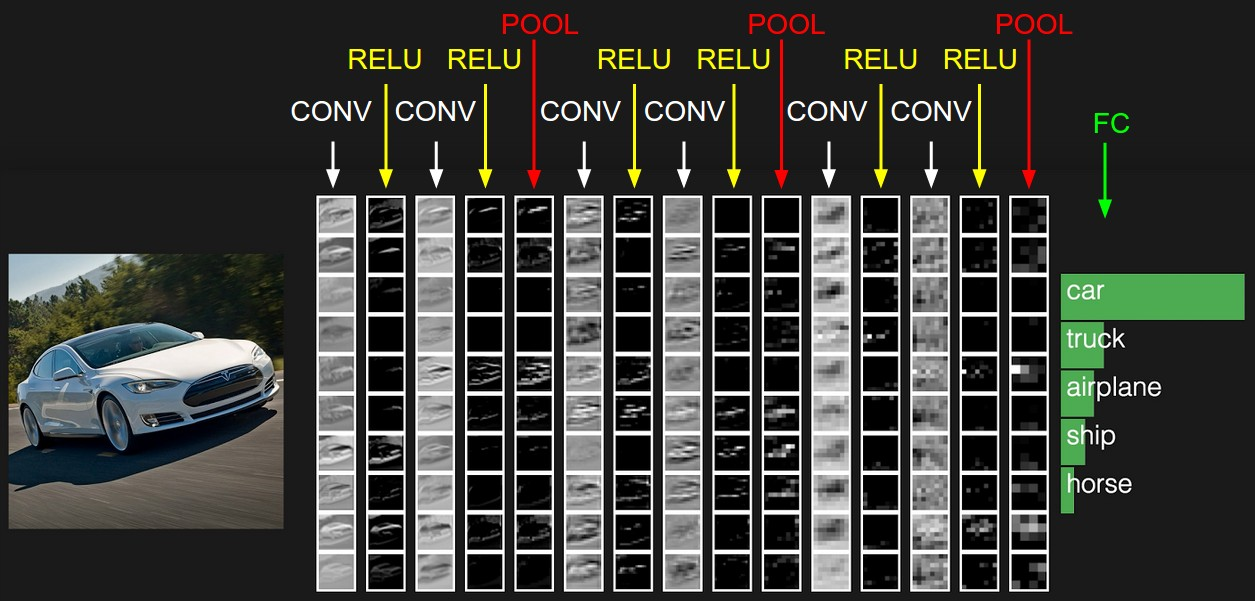
\includegraphics[width=8cm]{figures/convnet}
    \end{center}
    \caption{Example CNN Task}
    \label{fig:CNN}
\end{figure}

\subsection{Residual Blocks}
A traditional view of deep learning is that using a deeper network not necessarily results in better 
performance, in fact, simply stacking too many CNN blocks has been shown to cause a negative effect
since the gradient can easily shrink to zero. However, the ResNet with residual blocks brought by He et al. 
\cite{he2015deep} has eliminated this problem. The residual block skip connects between layers which adds
the output from previous layers $x$ to the output of stacked layers $F(x)$, in this way, even if something wrong
happens to the stacked deeper layers output(e.g. gradient vanishing), the network is still able to learn the 
identity output from the previous output. Therefore, residual blocks guarantee us to get results no worse than
a shallow network, and when this apply to CNN, a even deeper CNN can be more powerful for computer vision tasks.
\begin{figure}[H]
    \begin{center}
    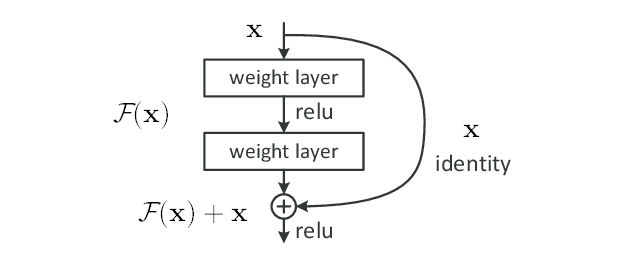
\includegraphics[width=8cm]{figures/resnet}
    \end{center}
    \caption{Structure of Residual Layer}
    \label{fig:Res-structure}
\end{figure}

\subsection{Batch Normalization}
\label{sec:BN}
Batch Normalization(BN) is a popular technique proposed by Ioffe and Szegedy \cite{ioffe2015batch} recently 
which alleviates a lot of headaches with properly initializing neural networks by forcing 
the activations throughout a network 
to take on a unit gaussian distribution at the beginning of the training according to \cite{cs231n}.
In deep learning, the latter layer could get inputs with a high variance and a mean value far from zero from the previous layer,
which is not good for stable training, to fix this problem, BN process every data with the equation:
$$y_{i}=\gamma \hat{x}_{i}+\beta \text { and } \hat{x}_{i}=\frac{x_{i}-\mu}{\sqrt{\sigma^{2}+\epsilon}}$$
Where $x_{i}$ is an activation for the $i^{th}$ example in the batch and $\hat{x}_{i}$ is the output after 
the process, $\mu$ and $\sigma^{2}$ are the mean value and variance of the activation over the batch, and
$\gamma$ and $\beta$ are trainable parameters.

In practice, we usually insert the BN layer between FC and non-linearities.
It has been shown that BN can make networks more robust to inappropriate
initialization. In addition, BN can be interpreted as doing preprocessing at every layer of a network, but 
integrated into the network itself in a differentiable manner, which is why BN is widely used nowadays.
For more details, please check the referenced paper \cite{ioffe2015batch}.

\section{Generative Adversarial Network}
Generative Adversarial Network(GAN) is one kind of deep learning approach originated from 
Goodfellow et al. \cite{goodfellow2014generative}. The idea of GAN is inspired from 
game theory: two neural networks contest against each other in a game(i.e. the training
process of deep learning), where one generator network tries to generate fake images while the 
other discriminator network tries to identify whether an image is real or fake. 
GAN models can learn
a loss that tries to classify if the output image is real or fake, while simultaneously training
a generative model to minimize this loss.
One advantage 
that GAN is more powerful than traditional CNN approach on image translation tasks is that 
GAN can produce clearer results for blurry images look obviously fake. Furthermore, we need 
expert knowledge and carefully designed loss function for traditional CNN models, while we 
only need to specify a high-level objective for GAN models: make the output looks like real, and then 
automatically learn a loss function for satisfying this goal, which is much more desirable.
\begin{figure}[H]
    \begin{center}
    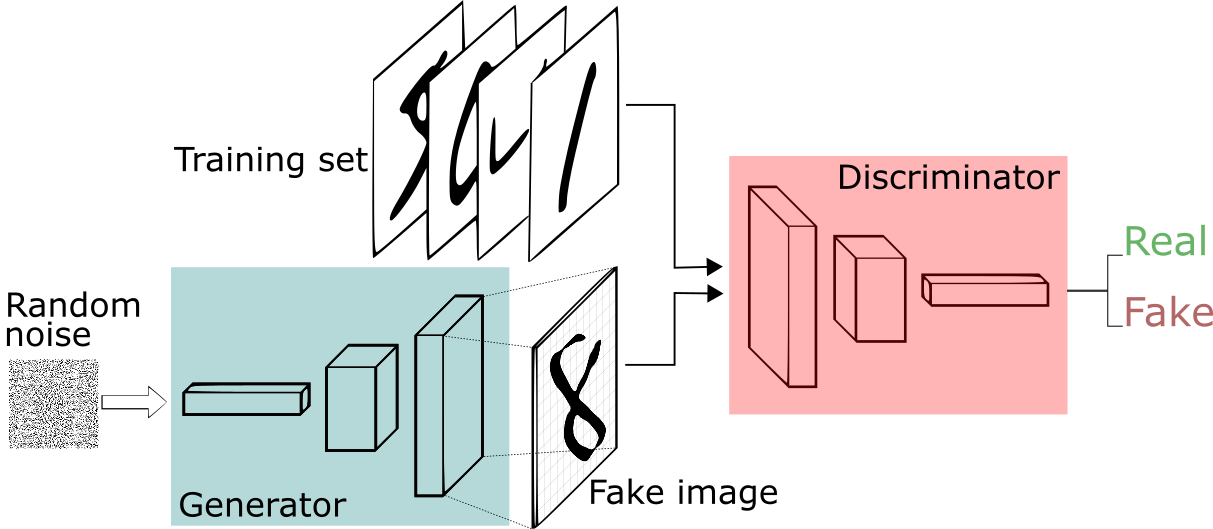
\includegraphics[width=8cm]{figures/GANs}
    \end{center}
    \caption{Structure of GANs}
    \label{fig:GANs-structure}
\end{figure}
\subsection{Conditional Generative Adversarial Network}
Conditional Generative Adversarial Network(cGAN) is a special kind of GAN whose input 
of the generator is not only the random noises, but also send in a condition image, the networks will learn 
to adapt and adjust their parameters to these additional condition inputs. For conventional GAN models, 
only the input noise can influence the output, however, for cGAN models, the conditional image can 
also influence the results. In image translation tasks, the encoded segmentation map is the condition 
we apply to the GAN model. Both pix2pix\cite{pix2pix2016} and pix2pixHD\cite{wang2018pix2pixHD} use 
this kind of GAN model.
\begin{figure}[H]
    \begin{center}
    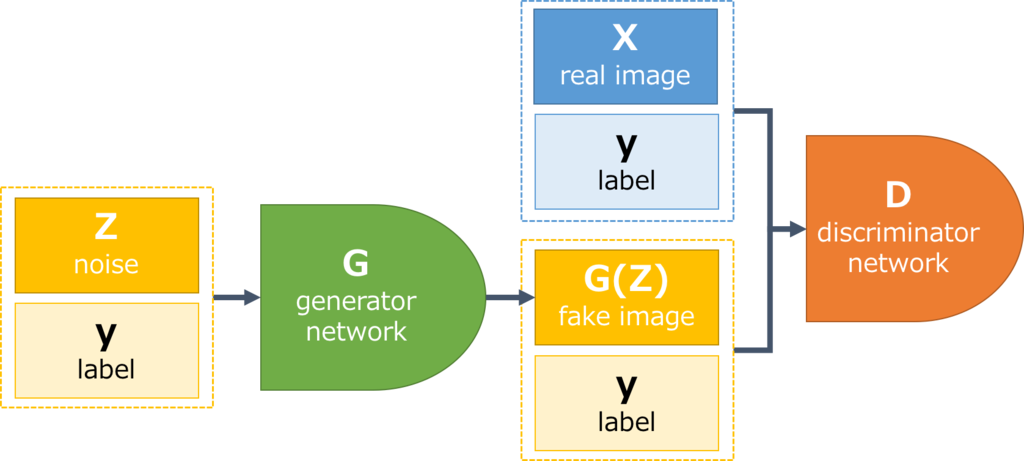
\includegraphics[width=8cm]{figures/cGANs}
    \end{center}
    \caption{Structure of conditional GANs}
    \label{fig:cGANs-structure}
\end{figure}

\section{Impact of COVID-19}
I decided to go back to Beijing after finishing my presentation of the 3rd year project on 16th March, 
my flight arrived at Xi'an, China at 23rd March, 
I had a low fever and was sent to a hospital for further checks, and fortunately, I am OK. 
After that, I was sent to a hotel and quarantine for 14 days in Xi'an, and then traveled back to Beijing and 
self-isolate for another 14 days at home according to the policies from the government. Generally speaking, I 
had quarantine for a month before I can work on my work wholeheartedly. Fortunately, I finished my demonstration 
before I left and the deadlines of the 3rd year project and other coursework have also been extended.

% Everything below here is commented material which is used by the
% emacs tex support system called auctex. If you're not an emacs user
% you can safely ignore it. If you do use emacs you should take a look
% at the local emacs or LaTeX WWW pages for more on emacs support for
% LaTeX.

% Local Variables:
% mode: latex
% TeX-master: "report"
% End:


\chapter{Literature Review}
\label{cha:review}
In this chapter, I will introduce how solving these kinds of image-to-image
translation tasks with GANs are originated, how the following models trying 
to improve the results, as well as details of two state-of-the-art models.

\section{Image-to-Image Translation with cGAN}
Dealing Image-to-Image translation tasks with GANs originated from Isola et al.\cite{pix2pix2016}.
\section{State-of-the-art Model — Pix2pixHD}

\section{State-of-the-art Model — SPADE}



% Local Variables: 
% mode: latex
% TeX-master: "report"
% End: 

\chapter{Project Development}
In this chapter, I will introduce how the project is developed,
the development tools and computational resources that I use for 
development.

This project tries to implement the two state-of-the-art models and 
expand their scope of application from datasets to arbitrary drawing.
Therefore, the whole project consists of two parts, training the deep 
learning models and building GUI to show the capability of the models.
Since training deep learning networks requires high computation power 
especially Graphics Processing Units(GPUs), which is not available to 
my laptop, so the plan is to train the models on Google Colab with 
free a GPU to use and then download the models and build a web app locally.

\section{Computational Resources}
Colaboratory brought by Google, often referred as Google Colab, is a 
free online interactive environment as the form of a jupyter notebook,
where we can write our python code and execute like our local jupyter 
notebook, furthermore, Google Colab has already configured most of the 
libraries for data science and machine learning, and it also provides 
a free GPU for us to use(K80, T4, P4, P100 will be allocated randomly).
However, it does have some problems, for example, sessions can get 
disconnected and accounts can be banned for a long time continuously 
using the GPU. So my solution is to save the model checkpoints after 
certain epochs of training, since Colab allows users to mount their google drive, 
I set the checkpoints saving directory in google drive so that I can 
continue training when I get disconnected.
Despite these inconveniences, this is the best solution 
I can think of. 

\section{Deep Learning Framework}
The deep learning framework I choose for this project is PyTorch from Facebook Inc. 
Pytorch is the Python implementation of the famous framework Torch, which offers tensor computation 
with strong GPU acceleration and deep neural networks built on a tape-based autograd system 
and it has become more and more popular in academia recently. 
On the one hand, Pytorch is friendly to tyros for 
you can easily understand what the code is doing and use the predefined 
frequently-used layers such as convolution layers, batch normalization layers, 
etc. On the other hand, it allows researchers to build deep neural networks with complex 
architectures flexibly which is an advantage over popular frameworks like Keras.
Unlike Tensorflow, Pytorch uses a dynamic computation graph instead 
of a static computation graph which is beneficial for tweaking and debugging. And 
the most important advantage of Pytorch over Tensorflow for me is that Pytorch 
has better documentation than Tensorflow, for example, you may find several 
functions doing the thing under different packages in Tensorflow documentation,
which is kind of chaos. For more information about Pytorch please visit 
\href{https://pytorch.org/}{https://pytorch.org/}.

\section{Graphical User Interface}
I decided to use a web page as the graphical user interface(GUI) for my project.
Unlike C++ or $C\sharp$, Python does not have any powerful desktop application GUI 
frameworks, however, 
web development tools like Flask and Django for Python can easily integrate the Pytorch 
library and can also make use of the front-end technology to make decent-looking 
GUI with their template system. 
When the user performs an action on the GUI, the front-end will send a request to 
the back-end, and the Flask framework will handle the request and ask Pytorch model to 
do the image translation if necessary. 

The front-end is basically developed with HTML, 
CSS, JavaScript, and libraries such as Bootstrap and Font Awesome.
In terms of back-end, I chose Flask, which is a lightweight WSGI web application 
framework for python. Flask projects start with a quick and easy setup but can scale 
up to complex applications, it also wraps Jinja2 which is a full-featured template 
engine that allows developers to integrate with front-end. 

The web app including 4 pages including a home page, an about page, two pages demonstrating
the capability of the model for translating segmentation maps in the dataset and arbitrary 
drawing semantic label maps respectively. 

\begin{figure}[H]
    \begin{center}
    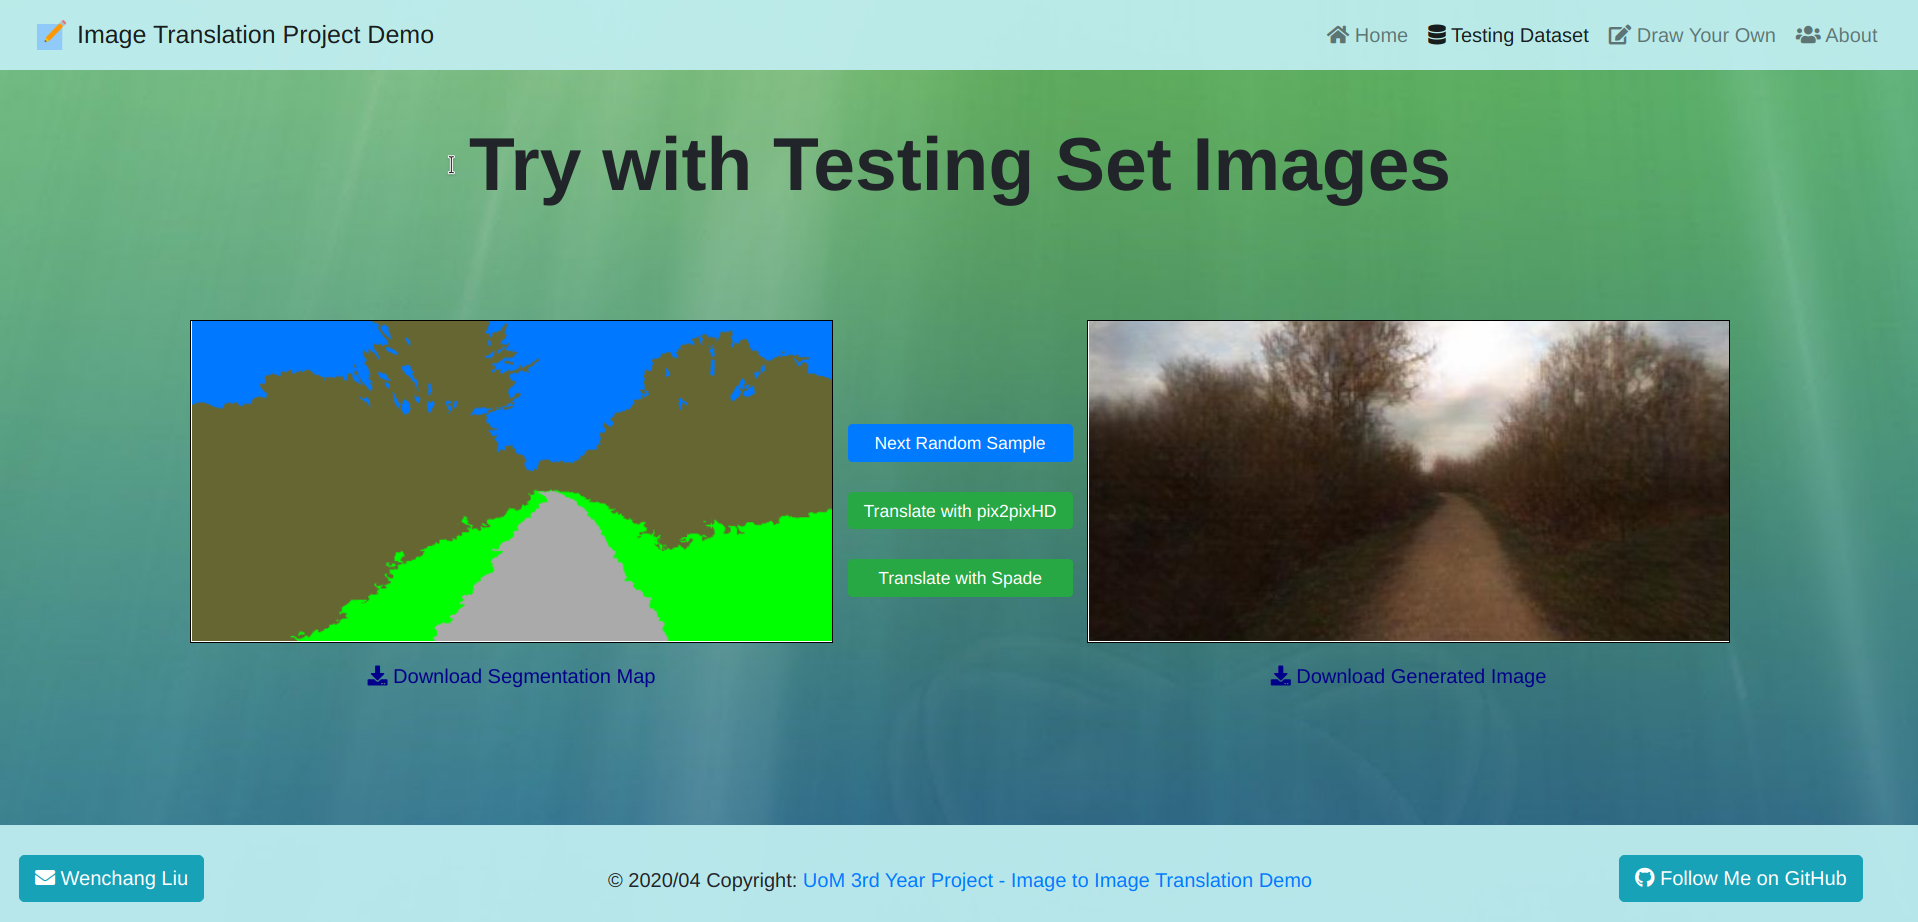
\includegraphics[width=14cm]{figures/GUI-testset}
    \end{center}
    \caption{Screenshot of the web page that allow users to try translating segmentation maps from the test dataset}
    \label{fig:GUI-testset}
\end{figure}

\begin{figure}[H]
    \begin{center}
    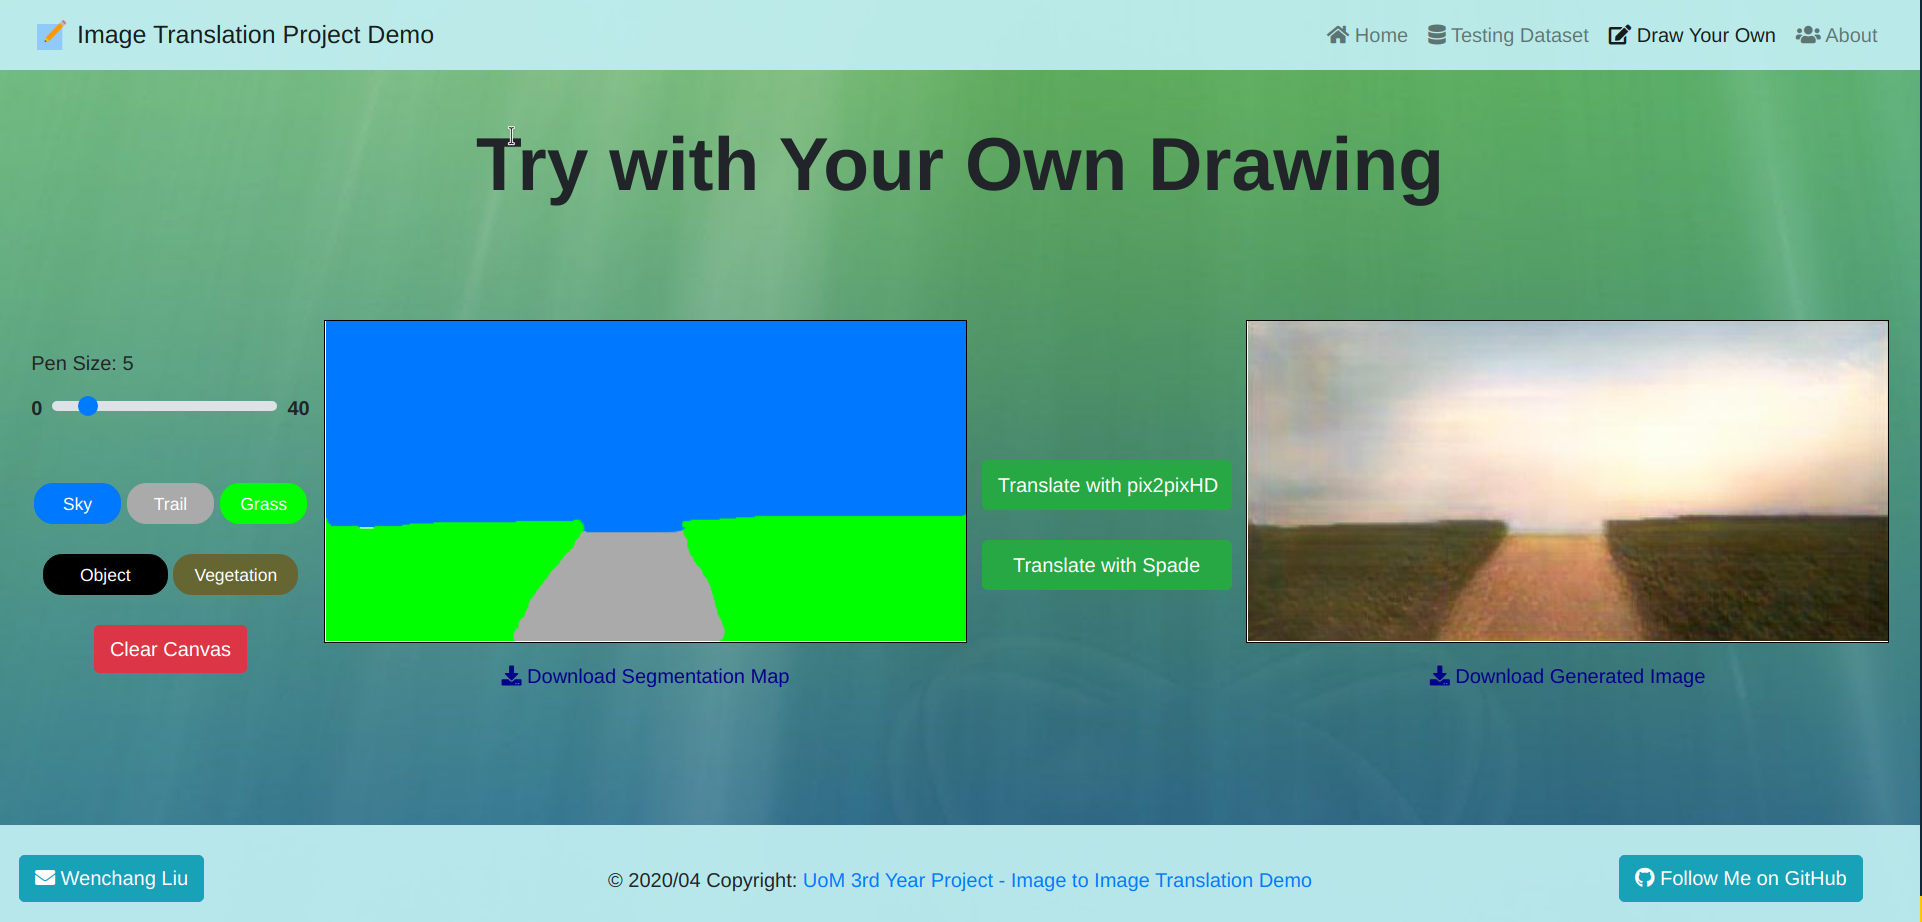
\includegraphics[width=14cm]{figures/GUI-draw}
    \end{center}
    \caption{Screenshot of the web page that allow users to try translating segmentation maps drawn by themselves}
    \label{fig:GUI-draw}
\end{figure}

As shown in figure \ref{fig:GUI-testset} and figure \ref{fig:GUI-testset}, 
the web app offers functionalities including getting next random sample segmentation map from 
the test dataset, a simple drawing tool for users to draw their own segmentation maps, 
downloading segmentation maps or generated photorealistic images, and translating the segmentation
map into photorealistic with both pix2pixHD and SPADE model.

The usage is so simple that all you need to do is get the segmentation map 
at the left(either by sampling from testing set or drawing one), press either of the 
translate buttons, and the photorealistic image will be appear at the right.


% Local Variables: 
% mode: latex
% TeX-master: "report"
% End: 

\chapter{Experiments and Evaluation}
In this chapter, I demonstrate the implementation details of the two state-of-the-art models, 
along with the experiments' results and evaluation. Due to the large number of training time 
of these state-of-the-art models and the limited computing resources(one free GPU from Colab), 
I decided to use one simpler dataset \cite{valada16iser} instead of the benchmark datasets 
for my project. In addition, most of the experiments were conducted in Pix2pixHD because 
the only difference for Pix2pixHD and SPADE is the generator, it is not necessary to carry 
out the experiments again on SPADE again.

\section{Dataset}
During the training of Pix2pixHD model, I experimented several different datasets, including 
benchmark datasets such as ADE20K\cite{zhou2017scene} and Cityscapes\cite{Cordts2016Cityscapes}, 
the simpler and smaller freiburg forest dataset \cite{valada16iser}. Based on my experiments, 
the freiburg forest dataset \cite{valada16iser} is more suitable for my project.
\subsection{Benchmark Datasets}
For image translation tasks, the training data we need are pairs of segmentation map and 
photorealistic images, which is exactly the same training data used for image segmentation 
tasks. Therefore, there are several popular benchmark datasets containing this kind of data, 
including coco-stuff\cite{caesar2018cvpr}, ADE20K\cite{zhou2017scene}, 
Cityscapes\cite{Cordts2016Cityscapes} which contain numerous 
classes of objects(e.g. Cityscapes have 30 classes of objects).
I have tried ADE20K and Cityscapes in the early stage of experiments:
\begin{itemize}
    \item ADE20K\cite{zhou2017scene} is a fully annotated image dataset designed for semantic segmentation, 
    there are 20210, 2000, 3000 images in the training, validation, testing set. All the 
    images in the training and validation set are annotated with objects with different 
    colors, many of them even get annotated with their parts. Unlike Cityscapes where 
    all the images are the scenes of cities, ADE20K covers various scenarios including 
    airfields, airports, houses, hospitals, etc. which makes the model even more 
    difficult to learn how to generate all these objects for they do not appear in the 
    similar environments. The size of this dataset is around 4GB.
    \item Cityscapes dataset\cite{Cordts2016Cityscapes} is a dataset focuses on semantic understanding of urban street 
    scenes including scenes from 50 cities, all seasons except winter, different 
    weather conditions, with 30 classes of objects. There are 5000 fine annotated 
    images for us to use. The real images are in high resolution so it is around 11GB
    large in total, also a large number of classes has also increased the difficulties 
    for our model to generate decent photorealistic images. 
\end{itemize}
If we want to achieve decent results on the testing set, we will 
have to train on all the images provided in the training set so that our model can adapt 
to different scenarios and learn the patterns of different kinds of objects. Nevertheless, 
even the smallest dataset among them has more than 4GB data, which makes each experiment 
of training lasts for days on the free GPU that Colab provides. This is the reason why 
in the project, I only use a small part of those data and keep the training time 
within an acceptable amount of time. 
\subsection{Freiburg Forest Dataset}
\label{sec:freiburg}
Freiburg Forest dataset\cite{valada16iser} was collected using an autonomous mobile robot equipped with 
cameras, where all scenes were recorded at 20HZ with $1024\times768$ resolution. The 
annotated images containing only 5 classes of objects including object, trail, grass, sky 
and vegetation, 230 pairs of images(each pair consists of a segmentation
map and a real photo) in the training set and 136 pairs of images in the testing set. 
The small scale of such dataset increases the fault tolerance for each training, i.e. I do 
not have to wait for hours to see the wrong intermediate results and start all over. 
Because the scenes are all similar and the objects are simple, so it does not need to train
on considerable training data to generate decent and clear images like the benchmark datasets,
which compensates the limited computing resources issue.
Even if this is a comparable small dataset, it still takes hours to train one single model. 
For downloading the annotated dataset(around 1GB) and more details, please 
check \href{http://deepscene.cs.uni-freiburg.de}{DeepScene} website.
\subsection{Preprocessing}
Pytorch allows us to load images from folders dynamically with “CustomDataset” function, so 
what I have to do is use “glob” function to find the pair of segmentation map and real photo 
image, and then use PIL library to corp the image into the required resolution(e.g. $512\times256$), 
and then return them to Pytorch.

Data augmentation techniques such as rotation or flipping can be applied, however, 
I do not see obvious improvement when I run the tutorial script of Pix2pix model, 
this is why I do not apply any of those to my implementation.

\section{Pix2pixHD Implementation}
The implementation of my Pix2pixHD basically follows the architecture from the paper, 
except I only uses 6 residual blocks instead of 9, you can see the architecture of the 
generator in figure \ref{fig:pix2pix-generator} and table \ref{Pix2pixHD generator table},  
the discriminator architecture in table \ref{Pix2pixHD discriminator table}. The final
solution is to train the networks with VGG loss on the Freiburg dataset with a
resolution of $512 \times 256$. Before that, 
I ran simulations on a small portion ADE20K to determine if the VGG loss component is 
effective or not. I also ran simulations on the Cityscapes dataset and tries to achieve similar 
results as the paper, but they all have some problems. 

Adam optimizer is used for training.
In terms of the learning rates, I set a higher learning rate for the generator instead of using 
identical learning rate because I noticed the discriminator loss can get down to a low value 
after just a few epochs of training while the generator merely reduce its loss a little 
each epoch, therefore, I hope I can speed up the training of the generator while keeping the 
discriminator as before. The generator learning rate $2\times10^{-5}$ and discriminator learning 
rate $10^{-5}$ seems to work fine for me. 

The whole GAN model training is a cyclic process, where for each epoch:
\begin{enumerate}
    \item Get a pair of images from the training dataset
    \item Generator generates a fake image according to input segmentation map
    \item Calculate discriminator loss(real loss, fake loss)
    \item Calculate generator loss(GAN loss, feature matching loss and VGG perceptual loss)
    \item Update weights of the models by backward pass
\end{enumerate}

\subsection{VGG Loss Experiment}
Even though in the paper the author claims that VGG loss does not have a significant influence on 
the generated image, I found the opposite conclusion when training the Pix2pixHD model on ADE20K 
dataset. In order to reduce the training time, I only uses air base images from ADE20K. 

At first, 
I did not use VGG loss component, the generator can learn to generate the shape of the objects 
however it cannot learn how to fill in the textures. As you can see in figure \ref{fig:without-VGG}, 
the generator can only learn the shape of the plane and people, but the generated picture 
consists of only two color mosaics.
\begin{figure}[H]
    \begin{center}
    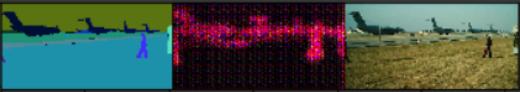
\includegraphics[width=10cm]{figures/without-VGG}
    \end{center}
    \caption{Example generated image without VGG loss during training}
    \label{fig:without-VGG}
\end{figure}

On the other hand, after adding the VGG loss component, the generator returns to normal, as you 
can see in figure \ref{fig:with-VGG}. Therefore, all simulations after this used VGG loss as well.
\begin{figure}[H]
    \begin{center}
    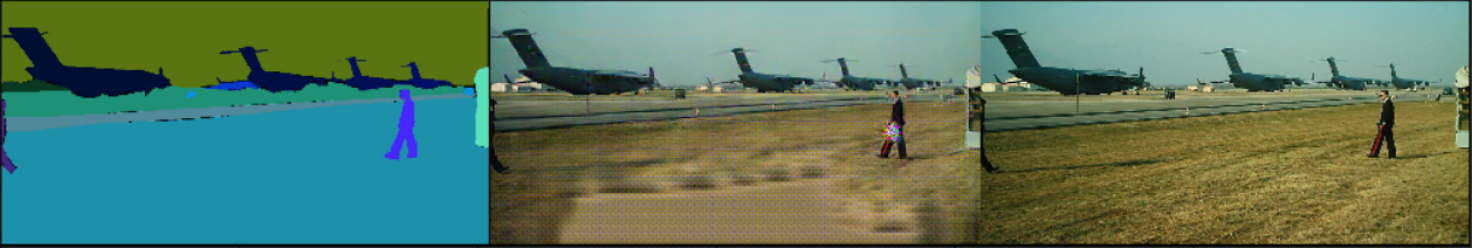
\includegraphics[width=10cm]{figures/with-VGG}
    \end{center}
    \caption{Example generated image with VGG loss during training}
    \label{fig:with-VGG}
\end{figure}

The VGG perceptual loss we use here is based on VGG-19\cite{articleVGG}, which is a very powerful
neural network trained for image classification. Using VGG loss means we compare the differences 
between the features extracted from the real images by a pre-trained VGG network and the features from 
the generator, since VGG network is very powerful, if our generator generates similar features as 
those from VGG, the final output should be excellent as well. The VGG perceptual loss has achieved 
marvelous results \cite{DBLP:journals/corr/JohnsonAL16} in style transfer tasks.     

Even with the help of VGG loss, merely using a few categories of images in ADE20K cannot achieve 
decent results when it comes to testing phases. As you can see in figure \ref{fig:ADE20K-test}, 
the model seemed to suffer from overfitting issue, i.e. the model performs quite well on 
a training set, but perform poorly at testing phases. This may because the training data is not 
enough, for example, during the training phase, the generator never encounter enough patterns of 
a person in front of the camera, so it does not know what pattern it should fill into that 
shape, that is why we can only see mosaics. Next, I experimented with several cities images 
from the Cityscapes dataset for all images in Cityscapes dataset describe the similar scenes, 
which is easier for our model to learn the patterns.
\begin{figure}[H]
    \begin{center}
    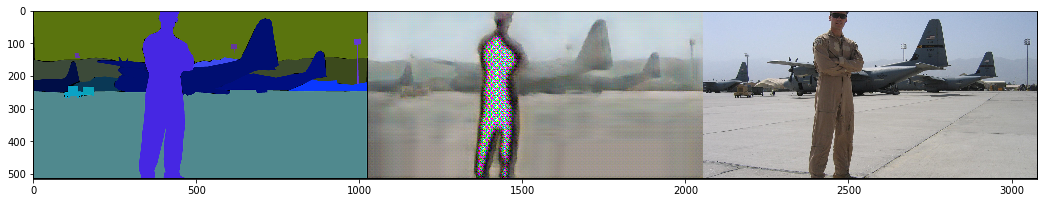
\includegraphics[width=10cm]{figures/ade20k-test}
    \end{center}
    \caption{Example generated image during testing phase with ADE20K air base images}
    \label{fig:ADE20K-test}
\end{figure}

\subsection{Cityscapes Experiment}
I spent a lot of time running simulation on Cityscapes dataset, despite I used only 3000 
pairs of images out of 5000. For the local enhancer, it took about 500 seconds for one 
epoch. The following figures \ref{fig:Cityscapes-train} \ref{fig:Cityscapes-test} are my 
results after 500 epochs of training on the global generator and 200 epochs of training 
on local enhancer, we can still observe the overfitting kind of issue as the training 
results look very realistic while the testing results have blur patterns everywhere 
which does not look real to me.
\begin{figure}[H]
    \begin{center}
    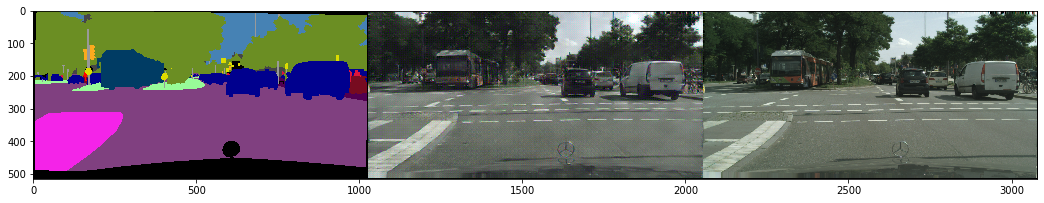
\includegraphics[width=14cm]{figures/cityscapes-train}
    \end{center}
    \caption{Example generated image during training phase with part of Cityscapes}
    \label{fig:Cityscapes-train}
\end{figure}

\begin{figure}[H]
    \begin{center}
    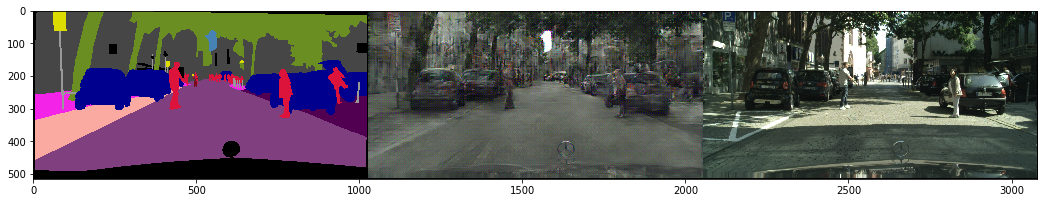
\includegraphics[width=14cm]{figures/cityscapes-test}
    \end{center}
    \caption{Example generated image during testing phase with part of Cityscapes}
    \label{fig:Cityscapes-test}
\end{figure}

Comparing the testing results with the training results, we can see the testing results
are not as good as the training results.
Continuing to train for more epochs or adjusting the hyperparameters are not likely to fix 
this issue since the training results have already been good enough, so it is more like a 
overfitting issue than an underfitting issue. Increasing the amount of images used for 
training is very likely to help, however, the significant training time makes it too 
difficult to finish on Colab. The reason for all these is that Cityscapes dataset contains 
too many classes of objects, and some class of objects have complex textures, which requires 
our model to learn from more training image if we want to generate them correctly without too 
many blurs.
This is why I decided to use a Cityscapes like dataset(i.e. single scenario) with 
fewer classes of objects and simpler textures for each class of objects, and the freiburg 
forest dataset just meets all the requirements.
\subsection{Train on Freiburg Forest Dataset}
We have already introduced freiburg forest dataset in \ref{sec:freiburg}. I trained the 
global generator for 200 epochs first, the training remain stable even we increase the 
learning rate for the generator which seems to be a success. I tracked the loss of the 
generator and discriminator for each epoch and figure \ref{fig:global-generator-loss} is the 
curve chart of the loss values for global generator and discriminator, which looks 
making sense. 
\begin{figure}[H]
    \begin{center}
    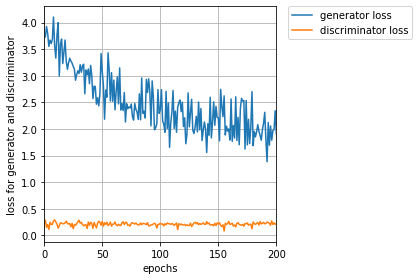
\includegraphics[width=8cm]{figures/global-generator-loss}
    \end{center}
    \caption{Loss values curve of global generator and discriminator during training}
    \label{fig:global-generator-loss}
\end{figure}
The global generator can generate decent images even when at testing phase, however,
we do observe many “dots” around the generated image as figure \ref{fig:global-generator-output}, 
this can be alleviated after 
we trained for certain epochs for the local enhancer.
\begin{figure}[H]
    \begin{center}
    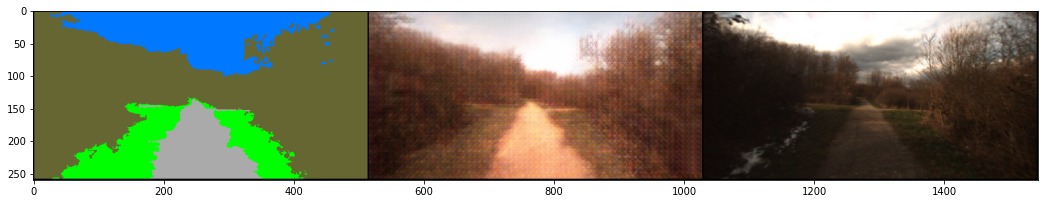
\includegraphics[width=14cm]{figures/global-generator-output}
    \end{center}
    \caption{Example output from Pix2pixHD global generator during testing}
    \label{fig:global-generator-output}
\end{figure}

I trained 100 epochs(about 4-5 hours) for local enhancer and it can already produce 
high quality images as figure \ref{fig:local-enhancer-output}. 
Since local enhancer aims to generate high resolution images, it alleviates the 
“dots” problem mentioned in global generator significantly.
Even you may still observe some blurs in certain areas, the overall quality is 
acceptable given the computing resources and training time we spent.
All the training parameters remain unchanged, and the training is also very stable, 
as you can see from figure \ref{fig:local-enhancer-loss}.
\begin{figure}[H]
    \begin{center}
    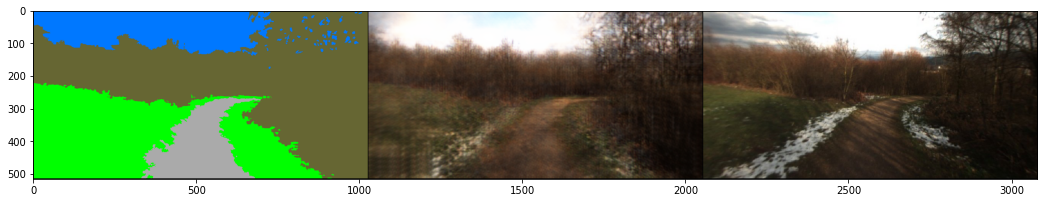
\includegraphics[width=14cm]{figures/local-enhancer-output}
    \end{center}
    \caption{Example output from Pix2pixHD local enhancer during testing}
    \label{fig:local-enhancer-output}
\end{figure}

\begin{figure}[H]
    \begin{center}
    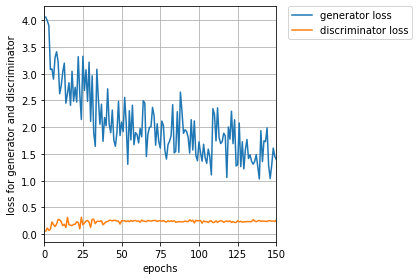
\includegraphics[width=8cm]{figures/local-enhancer-loss}
    \end{center}
    \caption{Loss values curve of local enhancer and discriminator during training}
    \label{fig:local-enhancer-loss}
\end{figure}

\subsection{Experiment Summary}
The table \ref{experimental results on Pix2pixHD} is the summary of the simulations that I ran with Pix2pixHD model, 
the results are consistent on multiple simulations:
\begin{table}[H]
    \begin{center}
    \begin{tabular}{|l|l|l|l|l|}\hline\hline
    Dataset&With/Without VGG&Stable Training&Training results&Testing results\\
    \hline
    ADE20K&Without VGG&Yes&Not Good&Not Good\\
    ADE20K&With VGG&Yes&Good&Not Good\\
    Cityscapes&With VGG&Yes&Good&Not Good\\
    Freiburg Forest&With VGG&Yes&Good&Good\\
    \hline\hline
    \end{tabular}
    \end{center}
    \caption{Experimental results on Pix2pixHD model}
    \label{experimental results on Pix2pixHD}
\end{table}

\section{SPADE Implementation}
\nocite{SPADE-blog-1}
\nocite{SPADE-blog-2}
SPADE is proposed after Pix2pixHD, which is trying to improve the results of Pix2pixHD further. 
The paper of SPADE provided the implementation of the networks in detail, so it is not 
a very difficult task to build the generator, also, apart from the generator, we can use the same 
code as Pix2pixHD implementation since they follow the same structure of GAN training.
\subsection{Generator of SPADE}
The generator of SPADE can be directly built according to the “Additional Implementation Details”
in the paper \cite{park2019SPADE} by stacking the building blocks. The order of building 
such networks is to build the SPADE block first, and then use SPADE blocks to build SPADE residual 
blocks, and in the end we can integrate SPADE residual blocks with the traditional GAN generator 
structure to build the SPADE generator. Note we use $512\times256$ resolution images, 
instead of $256\times256$ in the original paper, so we need 
to make small changes in terms of the tensor shapes, 
the general structure of the generator is showed with figure \ref{fig:SPADE-imp-generator}, 
and you can also check the final network structure with table \ref{SPADE generator table}. 
\begin{figure}
    \begin{center}
    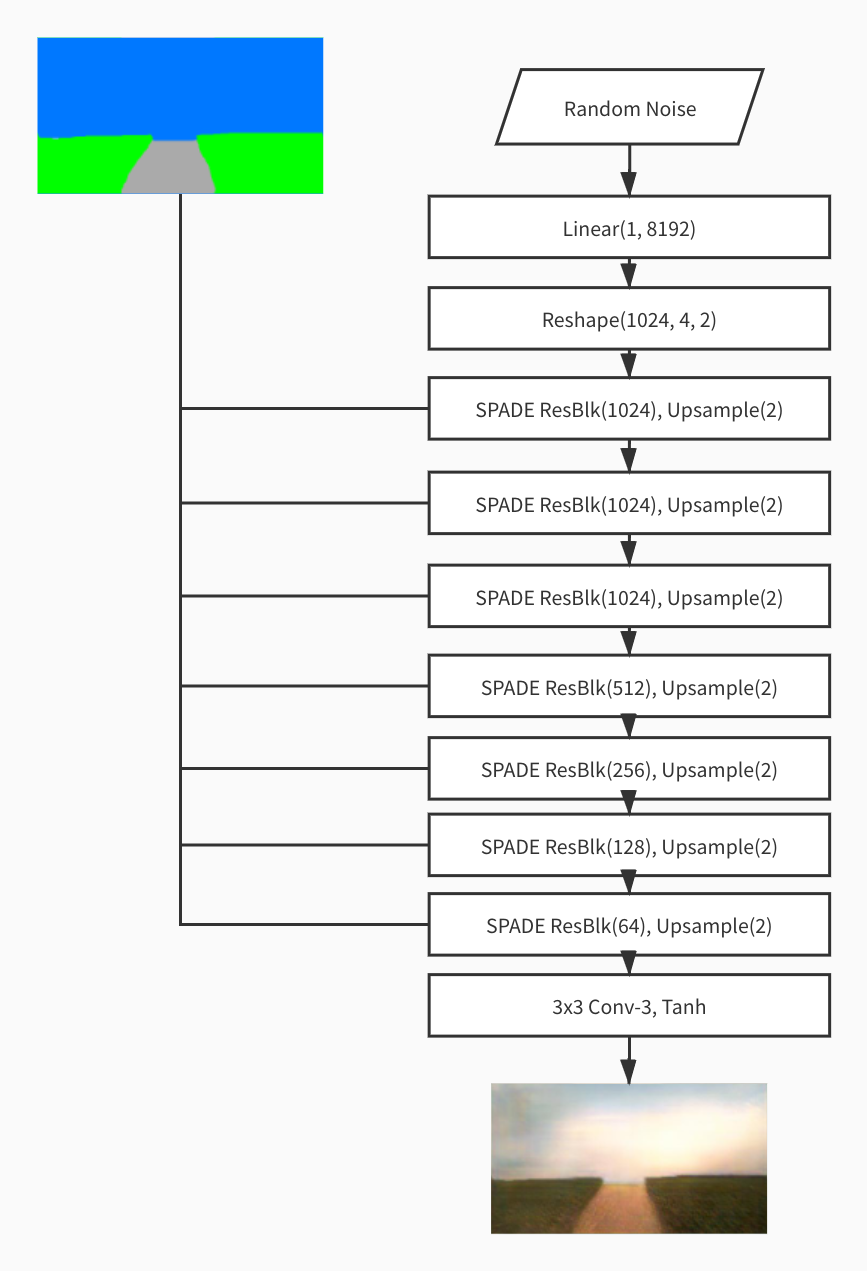
\includegraphics[width=8cm]{figures/SPADE-imp-generator}
    \end{center}
    \caption{SPADE Generator for Freiburg Forest Dataset}
    \label{fig:SPADE-imp-generator}
\end{figure} 

As shown in figure \ref{fig:SPADE-imp-generator}, the generation process is like we first 
generate random input noises shaped (1, 8192) for the batch size we use is one, we then 
reshape 8192 into (1024, 4, 2), next, the input noises will go through seven SPADE residual blocks 
together with the segmentation map, the output tensor will be upsampled 
by 2 after each SPADE residual block, eventually, a convolution layer with tanh activation 
will convert the tensor into images. You can refer to the SPADE block and SPADE residual block 
structure that the generator depends on in figure \ref{fig:SPADE-Block} and 
figure \ref{fig:SPADE-ResBlock} in chapter 2.
\subsection{Training}
The training configuration remained the same as Pix2pixHD, the only significant difference between 
these two model is the generator. I trained the SPADE model for 150 epochs and it can produce 
clear photorealistic images as figure \ref{fig:SPADE-output}. The loss value curve of 
the SPADE model training is also stable, the loss of the generator went down gradually as shown 
in figure \ref{fig:SPADE-loss}. 
\begin{figure}
    \begin{center}
    \includegraphics[width=14cm]{figures/SPADE-output}
    \end{center}
    \caption{Example output from SPADE generator during testing}
    \label{fig:SPADE-output}
\end{figure}
\begin{figure}
    \begin{center}
    \includegraphics[width=8cm]{figures/SPADE-loss}
    \end{center}
    \caption{Loss values curve of SPADE generator during training}
    \label{fig:SPADE-loss}
\end{figure}
We can see from table \ref{experimental results on SPADE} that the generator learns the correct way to generate images better 
and better as we trained it with more and more epochs, the improvement is significant from 1 to 
45 epochs, after that, the generator improves slower.
\begin{table}[H]
    \begin{center}
    \begin{tabular}{|l|l|l|}\hline\hline
    Epochs&Generator Loss&Testing Results\\
    \hline
    1&3.118682861328125&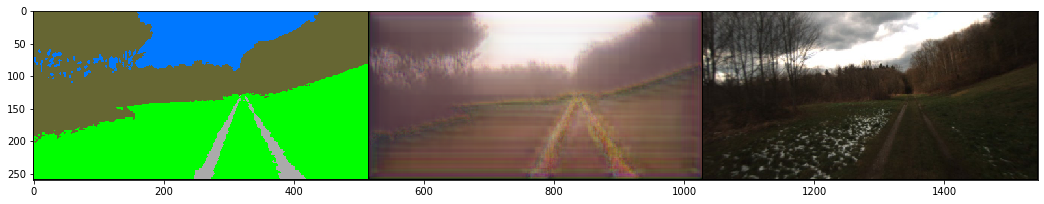
\includegraphics[width=8cm]{figures/spade-epoch-1}\\
    15&2.3608477115631104&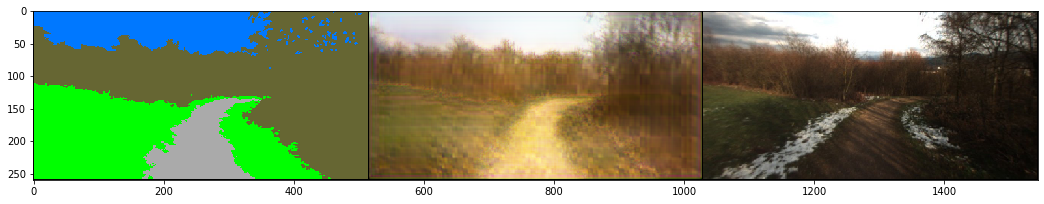
\includegraphics[width=8cm]{figures/spade-epoch-15}\\
    30&2.2259953022003174&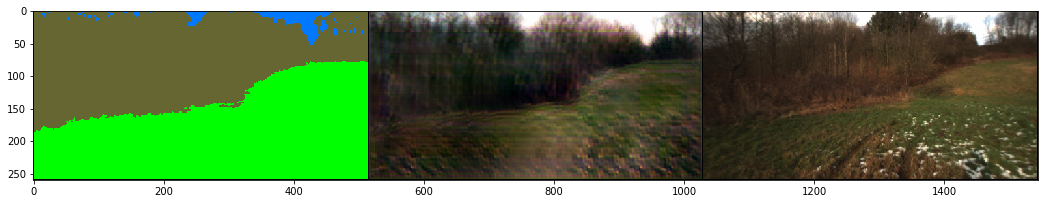
\includegraphics[width=8cm]{figures/spade-epoch-30}\\
    45&1.8741878271102905&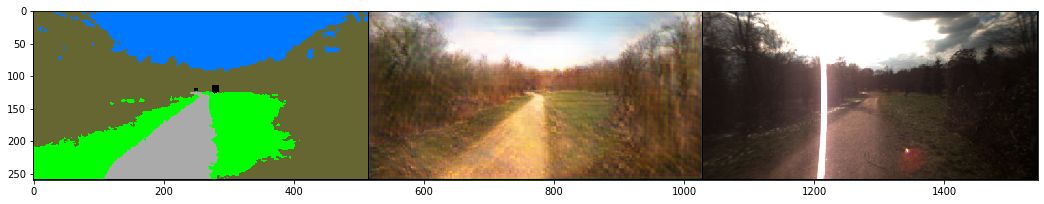
\includegraphics[width=8cm]{figures/spade-epoch-45}\\
    60&1.6682815551757812&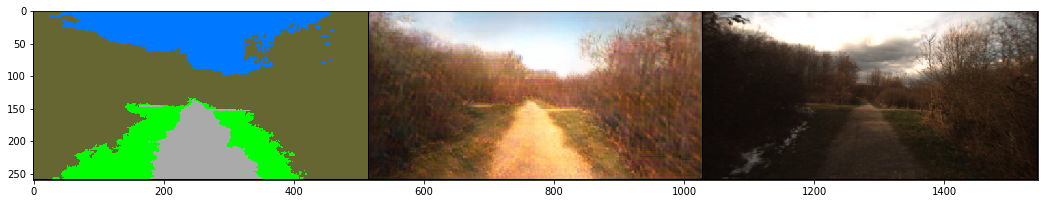
\includegraphics[width=8cm]{figures/spade-epoch-60}\\
    75&1.5951969623565674&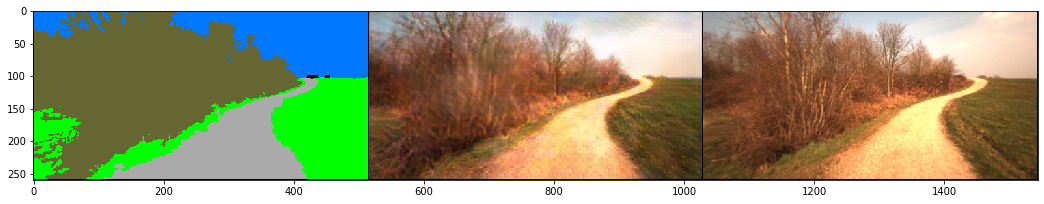
\includegraphics[width=8cm]{figures/spade-epoch-75}\\
    150&1.4927189350128174&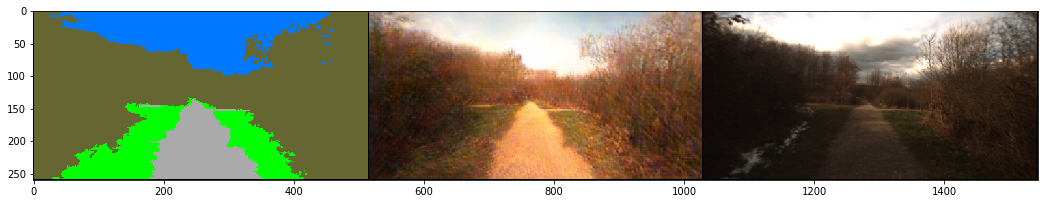
\includegraphics[width=8cm]{figures/spade-epoch-150}\\
    \hline\hline
    \end{tabular}
    \end{center}
    \caption{Experimental results on SPADE model}
    \label{experimental results on SPADE}
\end{table}

\section{Comparison}
If we compare the results of the Pix2pixHD model(figure \ref{fig:local-enhancer-output}) and 
SPADE model(figure \ref{fig:SPADE-output}), we might find SPADE model has the following 
advantages over Pix2pixHD: 
\begin{itemize}
    \item Clearer images without any “dot”: although the generated images are not perfectly 
    clear without any blur, it does remove the “dots” observed in the output of Pix2pixHD 
    model. We need more training data and more training time if we want to learn the textures 
    better of each class of objects.
    \item Only need to train one generator: when doing the implementation, I found training the 
    two generators for Pix2pixHD model really annoying, two generators' training require more 
    overall training time than one more complex model.
    \item Possibility of applying style transfer: since in the SPADE model, we no longer uses 
    conditional GAN structure for the generator, we remove the encoder part of the conditional 
    GAN generator, which adds the possibility of building another encoder that can encode a 
    style image and achieve style transfer effects. I have not implemented this feature which I 
    discuss further in section \ref{sec:future work}.
\end{itemize}

Nevertheless, the Pix2pixHD model is still the state-of-the-art model because it offers a way for 
us to generate high-resolution images. The SPADE model also takes more memory and longer time 
in the testing phase. The SPADE model can be used for higher resolution image 
translation in theory, but it has already needed a lot of training time, generating high-resolution 
images will require even more training time. 
\chapter{Reflection and Conclusion}

\bibliography{refs}             % this causes the references to be
                                % listed

\bibliographystyle{alpha}       % this determines the style in which
                                % the references are printed, other
                                % possible values are plain and abbrv
%% Appendices start here
\appendix
\section{附录:模型概述信息}
本附录包含了项目实现的两个生成器和一个辨别器神经网络的模型概述信息,由微软的tensorwatch开源软件生成。
具体的代码实现将会开源至我的\href{https://github.com/williamlwclwc}{GitHub}. 

\textbf{Pix2pixHD生成器结构概述信息}
\begin{longtable}{llll}
    \toprule
                        module name &        input shape &       output\_shape &  parameters \\
    \midrule
                    model\_global.0 &   (1, 3, 256, 128) &   (1, 3, 262, 134) &           0 \\
                    model\_global.1 &   (1, 3, 262, 134) &  (1, 64, 256, 128) &       9,472 \\
                    model\_global.2 &  (1, 64, 256, 128) &  (1, 64, 256, 128) &         128 \\
                    model\_global.3 &  (1, 64, 256, 128) &  (1, 64, 256, 128) &           0 \\
                    model\_global.4 &  (1, 64, 256, 128) &  (1, 128, 128, 64) &      73,856 \\
                    model\_global.5 &  (1, 128, 128, 64) &  (1, 128, 128, 64) &         256 \\
                    model\_global.6 &  (1, 128, 128, 64) &  (1, 128, 128, 64) &           0 \\
                    model\_global.7 &  (1, 128, 128, 64) &   (1, 256, 64, 32) &     295,168 \\
                    model\_global.8 &   (1, 256, 64, 32) &   (1, 256, 64, 32) &         512 \\
                    model\_global.9 &   (1, 256, 64, 32) &   (1, 256, 64, 32) &           0 \\
                    model\_global.10 &   (1, 256, 64, 32) &   (1, 512, 32, 16) &   1,180,160 \\
                    model\_global.11 &   (1, 512, 32, 16) &   (1, 512, 32, 16) &       1,024 \\
                    model\_global.12 &   (1, 512, 32, 16) &   (1, 512, 32, 16) &           0 \\
        model\_global.13.conv\_block.0 &   (1, 512, 32, 16) &   (1, 512, 34, 18) &           0 \\
        model\_global.13.conv\_block.1 &   (1, 512, 34, 18) &   (1, 512, 32, 16) &   2,359,808 \\
        model\_global.13.conv\_block.2 &   (1, 512, 32, 16) &   (1, 512, 32, 16) &       1,024 \\
        model\_global.13.conv\_block.3 &   (1, 512, 32, 16) &   (1, 512, 32, 16) &           0 \\
        model\_global.13.conv\_block.4 &   (1, 512, 32, 16) &   (1, 512, 34, 18) &           0 \\
        model\_global.13.conv\_block.5 &   (1, 512, 34, 18) &   (1, 512, 32, 16) &   2,359,808 \\
        model\_global.13.conv\_block.6 &   (1, 512, 32, 16) &   (1, 512, 32, 16) &       1,024 \\
        model\_global.14.conv\_block.0 &   (1, 512, 32, 16) &   (1, 512, 34, 18) &           0 \\
        model\_global.14.conv\_block.1 &   (1, 512, 34, 18) &   (1, 512, 32, 16) &   2,359,808 \\
        model\_global.14.conv\_block.2 &   (1, 512, 32, 16) &   (1, 512, 32, 16) &       1,024 \\
        model\_global.14.conv\_block.3 &   (1, 512, 32, 16) &   (1, 512, 32, 16) &           0 \\
        model\_global.14.conv\_block.4 &   (1, 512, 32, 16) &   (1, 512, 34, 18) &           0 \\
        model\_global.14.conv\_block.5 &   (1, 512, 34, 18) &   (1, 512, 32, 16) &   2,359,808 \\
        model\_global.14.conv\_block.6 &   (1, 512, 32, 16) &   (1, 512, 32, 16) &       1,024 \\
        model\_global.15.conv\_block.0 &   (1, 512, 32, 16) &   (1, 512, 34, 18) &           0 \\
        model\_global.15.conv\_block.1 &   (1, 512, 34, 18) &   (1, 512, 32, 16) &   2,359,808 \\
        model\_global.15.conv\_block.2 &   (1, 512, 32, 16) &   (1, 512, 32, 16) &       1,024 \\
        model\_global.15.conv\_block.3 &   (1, 512, 32, 16) &   (1, 512, 32, 16) &           0 \\
        model\_global.15.conv\_block.4 &   (1, 512, 32, 16) &   (1, 512, 34, 18) &           0 \\
        model\_global.15.conv\_block.5 &   (1, 512, 34, 18) &   (1, 512, 32, 16) &   2,359,808 \\
        model\_global.15.conv\_block.6 &   (1, 512, 32, 16) &   (1, 512, 32, 16) &       1,024 \\
        model\_global.16.conv\_block.0 &   (1, 512, 32, 16) &   (1, 512, 34, 18) &           0 \\
        model\_global.16.conv\_block.1 &   (1, 512, 34, 18) &   (1, 512, 32, 16) &   2,359,808 \\
        model\_global.16.conv\_block.2 &   (1, 512, 32, 16) &   (1, 512, 32, 16) &       1,024 \\
        model\_global.16.conv\_block.3 &   (1, 512, 32, 16) &   (1, 512, 32, 16) &           0 \\
        model\_global.16.conv\_block.4 &   (1, 512, 32, 16) &   (1, 512, 34, 18) &           0 \\
        model\_global.16.conv\_block.5 &   (1, 512, 34, 18) &   (1, 512, 32, 16) &   2,359,808 \\
        model\_global.16.conv\_block.6 &   (1, 512, 32, 16) &   (1, 512, 32, 16) &       1,024 \\
        model\_global.17.conv\_block.0 &   (1, 512, 32, 16) &   (1, 512, 34, 18) &           0 \\
        model\_global.17.conv\_block.1 &   (1, 512, 34, 18) &   (1, 512, 32, 16) &   2,359,808 \\
        model\_global.17.conv\_block.2 &   (1, 512, 32, 16) &   (1, 512, 32, 16) &       1,024 \\
        model\_global.17.conv\_block.3 &   (1, 512, 32, 16) &   (1, 512, 32, 16) &           0 \\
        model\_global.17.conv\_block.4 &   (1, 512, 32, 16) &   (1, 512, 34, 18) &           0 \\
        model\_global.17.conv\_block.5 &   (1, 512, 34, 18) &   (1, 512, 32, 16) &   2,359,808 \\
        model\_global.17.conv\_block.6 &   (1, 512, 32, 16) &   (1, 512, 32, 16) &       1,024 \\
        model\_global.18.conv\_block.0 &   (1, 512, 32, 16) &   (1, 512, 34, 18) &           0 \\
        model\_global.18.conv\_block.1 &   (1, 512, 34, 18) &   (1, 512, 32, 16) &   2,359,808 \\
        model\_global.18.conv\_block.2 &   (1, 512, 32, 16) &   (1, 512, 32, 16) &       1,024 \\
        model\_global.18.conv\_block.3 &   (1, 512, 32, 16) &   (1, 512, 32, 16) &           0 \\
        model\_global.18.conv\_block.4 &   (1, 512, 32, 16) &   (1, 512, 34, 18) &           0 \\
        model\_global.18.conv\_block.5 &   (1, 512, 34, 18) &   (1, 512, 32, 16) &   2,359,808 \\
        model\_global.18.conv\_block.6 &   (1, 512, 32, 16) &   (1, 512, 32, 16) &       1,024 \\
                    model\_global.19 &   (1, 512, 32, 16) &   (1, 256, 64, 32) &   1,179,904 \\
                    model\_global.20 &   (1, 256, 64, 32) &   (1, 256, 64, 32) &         512 \\
                    model\_global.21 &   (1, 256, 64, 32) &   (1, 256, 64, 32) &           0 \\
                    model\_global.22 &   (1, 256, 64, 32) &  (1, 128, 128, 64) &     295,040 \\
                    model\_global.23 &  (1, 128, 128, 64) &  (1, 128, 128, 64) &         256 \\
                    model\_global.24 &  (1, 128, 128, 64) &  (1, 128, 128, 64) &           0 \\
                    model\_global.25 &  (1, 128, 128, 64) &  (1, 64, 256, 128) &      73,792 \\
                    model\_global.26 &  (1, 64, 256, 128) &  (1, 64, 256, 128) &         128 \\
                    model\_global.27 &  (1, 64, 256, 128) &  (1, 64, 256, 128) &           0 \\
                    model\_global.28 &                 [] &                 [] &           0 \\
                    model\_global.29 &                 [] &                 [] &           0 \\
                    model\_global.30 &                 [] &                 [] &           0 \\
                        downsample &   (1, 3, 512, 256) &   (1, 3, 256, 128) &           0 \\
                    le\_downsample.0 &   (1, 3, 512, 256) &   (1, 3, 518, 262) &           0 \\
                    le\_downsample.1 &   (1, 3, 518, 262) &  (1, 32, 512, 256) &       4,736 \\
                    le\_downsample.2 &  (1, 32, 512, 256) &  (1, 32, 512, 256) &          64 \\
                    le\_downsample.3 &  (1, 32, 512, 256) &  (1, 32, 512, 256) &           0 \\
                    le\_downsample.4 &  (1, 32, 512, 256) &  (1, 64, 256, 128) &      18,496 \\
                    le\_downsample.5 &  (1, 64, 256, 128) &  (1, 64, 256, 128) &         128 \\
                    le\_downsample.6 &  (1, 64, 256, 128) &  (1, 64, 256, 128) &           0 \\
        le\_upsample.0.conv\_block.0 &  (1, 64, 256, 128) &  (1, 64, 258, 130) &           0 \\
        le\_upsample.0.conv\_block.1 &  (1, 64, 258, 130) &  (1, 64, 256, 128) &      36,928 \\
        le\_upsample.0.conv\_block.2 &  (1, 64, 256, 128) &  (1, 64, 256, 128) &         128 \\
        le\_upsample.0.conv\_block.3 &  (1, 64, 256, 128) &  (1, 64, 256, 128) &           0 \\
        le\_upsample.0.conv\_block.4 &  (1, 64, 256, 128) &  (1, 64, 258, 130) &           0 \\
        le\_upsample.0.conv\_block.5 &  (1, 64, 258, 130) &  (1, 64, 256, 128) &      36,928 \\
        le\_upsample.0.conv\_block.6 &  (1, 64, 256, 128) &  (1, 64, 256, 128) &         128 \\
        le\_upsample.1.conv\_block.0 &  (1, 64, 256, 128) &  (1, 64, 258, 130) &           0 \\
        le\_upsample.1.conv\_block.1 &  (1, 64, 258, 130) &  (1, 64, 256, 128) &      36,928 \\
        le\_upsample.1.conv\_block.2 &  (1, 64, 256, 128) &  (1, 64, 256, 128) &         128 \\
        le\_upsample.1.conv\_block.4 &  (1, 64, 256, 128) &  (1, 64, 258, 130) &           0 \\
        le\_upsample.1.conv\_block.5 &  (1, 64, 258, 130) &  (1, 64, 256, 128) &      36,928 \\
        le\_upsample.1.conv\_block.6 &  (1, 64, 256, 128) &  (1, 64, 256, 128) &         128 \\
        le\_upsample.2.conv\_block.0 &  (1, 64, 256, 128) &  (1, 64, 258, 130) &           0 \\
        le\_upsample.2.conv\_block.1 &  (1, 64, 258, 130) &  (1, 64, 256, 128) &      36,928 \\
        le\_upsample.2.conv\_block.2 &  (1, 64, 256, 128) &  (1, 64, 256, 128) &         128 \\
        le\_upsample.2.conv\_block.4 &  (1, 64, 256, 128) &  (1, 64, 258, 130) &           0 \\
        le\_upsample.2.conv\_block.5 &  (1, 64, 258, 130) &  (1, 64, 256, 128) &      36,928 \\
        le\_upsample.2.conv\_block.6 &  (1, 64, 256, 128) &  (1, 64, 256, 128) &         128 \\
                    le\_upsample.3 &  (1, 64, 256, 128) &  (1, 32, 512, 256) &      18,464 \\
                    le\_upsample.4 &  (1, 32, 512, 256) &  (1, 32, 512, 256) &          64 \\
                    le\_upsample.5 &  (1, 32, 512, 256) &  (1, 32, 512, 256) &           0 \\
                    le\_upsample.6 &  (1, 32, 512, 256) &  (1, 32, 518, 262) &           0 \\
                    le\_upsample.7 &  (1, 32, 518, 262) &   (1, 3, 512, 256) &       4,707 \\
                    le\_upsample.8 &   (1, 3, 512, 256) &   (1, 3, 512, 256) &           0 \\
                            Model &   [1, 3, 512, 256] &   (1, 3, 512, 256) &  31,709,187 \\
    \bottomrule
    \caption{由tensorwatch生成的Pix2pixHD生成器模型概述信息}
    \label{Pix2pixHD generator table}
\end{longtable}  
    
\textbf{辨别器的模型结构概述信息}
\begin{table}[H]
    \begin{tabular}{llll}
        \toprule
        module name &        input shape &       output shape & parameters \\
        \midrule
        downsample &   (1, 6, 256, 128) &    (1, 6, 128, 64) &          0 \\
        layer0.0 &    (1, 6, 128, 64) &    (1, 64, 65, 33) &      6,208 \\
        layer0.1 &    (1, 64, 65, 33) &    (1, 64, 65, 33) &          0 \\
        layer0.2 &    (1, 64, 65, 33) &   (1, 128, 33, 17) &    131,200 \\
        layer0.3 &   (1, 128, 33, 17) &   (1, 128, 33, 17) &        256 \\
        layer0.4 &   (1, 128, 33, 17) &   (1, 128, 33, 17) &          0 \\
        layer0.5 &   (1, 128, 33, 17) &    (1, 256, 17, 9) &    524,544 \\
        layer0.6 &    (1, 256, 17, 9) &    (1, 256, 17, 9) &        512 \\
        layer0.7 &    (1, 256, 17, 9) &    (1, 256, 17, 9) &          0 \\
        layer0.8 &    (1, 256, 17, 9) &   (1, 512, 18, 10) &  2,097,664 \\
        layer0.9 &   (1, 512, 18, 10) &   (1, 512, 18, 10) &      1,024 \\
        layer0.10 &   (1, 512, 18, 10) &   (1, 512, 18, 10) &          0 \\
        layer0.11 &   (1, 512, 18, 10) &     (1, 1, 19, 11) &      8,193 \\
        layer1.0 &   (1, 6, 256, 128) &   (1, 64, 129, 65) &      6,208 \\
        layer1.1 &   (1, 64, 129, 65) &   (1, 64, 129, 65) &          0 \\
        layer1.2 &   (1, 64, 129, 65) &   (1, 128, 65, 33) &    131,200 \\
        layer1.3 &   (1, 128, 65, 33) &   (1, 128, 65, 33) &        256 \\
        layer1.4 &   (1, 128, 65, 33) &   (1, 128, 65, 33) &          0 \\
        layer1.5 &   (1, 128, 65, 33) &   (1, 256, 33, 17) &    524,544 \\
        layer1.6 &   (1, 256, 33, 17) &   (1, 256, 33, 17) &        512 \\
        layer1.7 &   (1, 256, 33, 17) &   (1, 256, 33, 17) &          0 \\
        layer1.8 &   (1, 256, 33, 17) &   (1, 512, 34, 18) &  2,097,664 \\
        layer1.9 &   (1, 512, 34, 18) &   (1, 512, 34, 18) &      1,024 \\
        layer1.10 &   (1, 512, 34, 18) &   (1, 512, 34, 18) &          0 \\
        layer1.11 &   (1, 512, 34, 18) &     (1, 1, 35, 19) &      8,193 \\
        layer2.0 &   (1, 6, 512, 256) &  (1, 64, 257, 129) &      6,208 \\
        layer2.1 &  (1, 64, 257, 129) &  (1, 64, 257, 129) &          0 \\
        layer2.2 &  (1, 64, 257, 129) &  (1, 128, 129, 65) &    131,200 \\
        layer2.3 &  (1, 128, 129, 65) &  (1, 128, 129, 65) &        256 \\
        layer2.4 &  (1, 128, 129, 65) &  (1, 128, 129, 65) &          0 \\
        layer2.5 &  (1, 128, 129, 65) &   (1, 256, 65, 33) &    524,544 \\
        layer2.6 &   (1, 256, 65, 33) &   (1, 256, 65, 33) &        512 \\
        layer2.7 &   (1, 256, 65, 33) &   (1, 256, 65, 33) &          0 \\
        layer2.8 &   (1, 256, 65, 33) &   (1, 512, 66, 34) &  2,097,664 \\
        layer2.9 &   (1, 512, 66, 34) &   (1, 512, 66, 34) &      1,024 \\
        layer2.10 &   (1, 512, 66, 34) &   (1, 512, 66, 34) &          0 \\
        layer2.11 &   (1, 512, 66, 34) &     (1, 1, 67, 35) &      8,193 \\
            Model &   [1, 6, 512, 256] &     (1, 1, 67, 35) &  8,308,803 \\
        \bottomrule
    \end{tabular}
    \caption{由tensorwatch生成的辨别器模型概述信息}
    \label{Pix2pixHD discriminator table}
\end{table}
    
\textbf{SPADE模型的生成器模型概述信息}
\begin{longtable}{llll}
    \toprule
                            module name &         input shape &        output shape &   parameters \\
    \midrule
                                    fc &            (1, 256) &           (1, 8192) &    2,105,344 \\
        spadeRes0.spade0.param\_free\_norm &     (1, 1024, 4, 2) &     (1, 1024, 4, 2) &            0 \\
            spadeRes0.spade0.shared\_net.0 &        (1, 3, 4, 2) &      (1, 128, 4, 2) &        3,584 \\
            spadeRes0.spade0.shared\_net.1 &      (1, 128, 4, 2) &      (1, 128, 4, 2) &            0 \\
                spadeRes0.spade0.gamma &      (1, 128, 4, 2) &     (1, 1024, 4, 2) &    1,180,672 \\
                    spadeRes0.spade0.beta &      (1, 128, 4, 2) &     (1, 1024, 4, 2) &    1,180,672 \\
                        spadeRes0.conv0 &     (1, 1024, 4, 2) &     (1, 1024, 4, 2) &    9,438,208 \\
                        spadeRes0.relu0 &     (1, 1024, 4, 2) &     (1, 1024, 4, 2) &            0 \\
        spadeRes0.spade1.param\_free\_norm &     (1, 1024, 4, 2) &     (1, 1024, 4, 2) &            0 \\
            spadeRes0.spade1.shared\_net.0 &        (1, 3, 4, 2) &      (1, 128, 4, 2) &        3,584 \\
            spadeRes0.spade1.shared\_net.1 &      (1, 128, 4, 2) &      (1, 128, 4, 2) &            0 \\
                spadeRes0.spade1.gamma &      (1, 128, 4, 2) &     (1, 1024, 4, 2) &    1,180,672 \\
                    spadeRes0.spade1.beta &      (1, 128, 4, 2) &     (1, 1024, 4, 2) &    1,180,672 \\
                        spadeRes0.conv1 &     (1, 1024, 4, 2) &     (1, 1024, 4, 2) &    9,438,208 \\
                        spadeRes0.relu1 &     (1, 1024, 4, 2) &     (1, 1024, 4, 2) &            0 \\
    spadeRes0.spade\_skip.param\_free\_norm &     (1, 1024, 4, 2) &     (1, 1024, 4, 2) &            0 \\
        spadeRes0.spade\_skip.shared\_net.0 &        (1, 3, 4, 2) &      (1, 128, 4, 2) &        3,584 \\
        spadeRes0.spade\_skip.shared\_net.1 &      (1, 128, 4, 2) &      (1, 128, 4, 2) &            0 \\
            spadeRes0.spade\_skip.gamma &      (1, 128, 4, 2) &     (1, 1024, 4, 2) &    1,180,672 \\
                spadeRes0.spade\_skip.beta &      (1, 128, 4, 2) &     (1, 1024, 4, 2) &    1,180,672 \\
                    spadeRes0.conv\_skip &     (1, 1024, 4, 2) &     (1, 1024, 4, 2) &    1,048,576 \\
                    spadeRes0.relu\_skip &     (1, 1024, 4, 2) &     (1, 1024, 4, 2) &            0 \\
        spadeRes1.spade0.param\_free\_norm &     (1, 1024, 8, 4) &     (1, 1024, 8, 4) &            0 \\
            spadeRes1.spade0.shared\_net.0 &        (1, 3, 8, 4) &      (1, 128, 8, 4) &        3,584 \\
            spadeRes1.spade0.shared\_net.1 &      (1, 128, 8, 4) &      (1, 128, 8, 4) &            0 \\
                spadeRes1.spade0.gamma &      (1, 128, 8, 4) &     (1, 1024, 8, 4) &    1,180,672 \\
                    spadeRes1.spade0.beta &      (1, 128, 8, 4) &     (1, 1024, 8, 4) &    1,180,672 \\
                        spadeRes1.conv0 &     (1, 1024, 8, 4) &     (1, 1024, 8, 4) &    9,438,208 \\
                        spadeRes1.relu0 &     (1, 1024, 8, 4) &     (1, 1024, 8, 4) &            0 \\
        spadeRes1.spade1.param\_free\_norm &     (1, 1024, 8, 4) &     (1, 1024, 8, 4) &            0 \\
            spadeRes1.spade1.shared\_net.0 &        (1, 3, 8, 4) &      (1, 128, 8, 4) &        3,584 \\
            spadeRes1.spade1.shared\_net.1 &      (1, 128, 8, 4) &      (1, 128, 8, 4) &            0 \\
                spadeRes1.spade1.gamma &      (1, 128, 8, 4) &     (1, 1024, 8, 4) &    1,180,672 \\
                    spadeRes1.spade1.beta &      (1, 128, 8, 4) &     (1, 1024, 8, 4) &    1,180,672 \\
                        spadeRes1.conv1 &     (1, 1024, 8, 4) &     (1, 1024, 8, 4) &    9,438,208 \\
                        spadeRes1.relu1 &     (1, 1024, 8, 4) &     (1, 1024, 8, 4) &            0 \\
    spadeRes1.spade\_skip.param\_free\_norm &     (1, 1024, 8, 4) &     (1, 1024, 8, 4) &            0 \\
        spadeRes1.spade\_skip.shared\_net.0 &        (1, 3, 8, 4) &      (1, 128, 8, 4) &        3,584 \\
        spadeRes1.spade\_skip.shared\_net.1 &      (1, 128, 8, 4) &      (1, 128, 8, 4) &            0 \\
            spadeRes1.spade\_skip.gamma &      (1, 128, 8, 4) &     (1, 1024, 8, 4) &    1,180,672 \\
                spadeRes1.spade\_skip.beta &      (1, 128, 8, 4) &     (1, 1024, 8, 4) &    1,180,672 \\
                    spadeRes1.conv\_skip &     (1, 1024, 8, 4) &     (1, 1024, 8, 4) &    1,048,576 \\
                    spadeRes1.relu\_skip &     (1, 1024, 8, 4) &     (1, 1024, 8, 4) &            0 \\
        spadeRes2.spade0.param\_free\_norm &    (1, 1024, 16, 8) &    (1, 1024, 16, 8) &            0 \\
            spadeRes2.spade0.shared\_net.0 &       (1, 3, 16, 8) &     (1, 128, 16, 8) &        3,584 \\
            spadeRes2.spade0.shared\_net.1 &     (1, 128, 16, 8) &     (1, 128, 16, 8) &            0 \\
                spadeRes2.spade0.gamma &     (1, 128, 16, 8) &    (1, 1024, 16, 8) &    1,180,672 \\
                    spadeRes2.spade0.beta &     (1, 128, 16, 8) &    (1, 1024, 16, 8) &    1,180,672 \\
                        spadeRes2.conv0 &    (1, 1024, 16, 8) &    (1, 1024, 16, 8) &    9,438,208 \\
                        spadeRes2.relu0 &    (1, 1024, 16, 8) &    (1, 1024, 16, 8) &            0 \\
        spadeRes2.spade1.param\_free\_norm &    (1, 1024, 16, 8) &    (1, 1024, 16, 8) &            0 \\
            spadeRes2.spade1.shared\_net.0 &       (1, 3, 16, 8) &     (1, 128, 16, 8) &        3,584 \\
            spadeRes2.spade1.shared\_net.1 &     (1, 128, 16, 8) &     (1, 128, 16, 8) &            0 \\
                spadeRes2.spade1.gamma &     (1, 128, 16, 8) &    (1, 1024, 16, 8) &    1,180,672 \\
                    spadeRes2.spade1.beta &     (1, 128, 16, 8) &    (1, 1024, 16, 8) &    1,180,672 \\
                        spadeRes2.conv1 &    (1, 1024, 16, 8) &    (1, 1024, 16, 8) &    9,438,208 \\
                        spadeRes2.relu1 &    (1, 1024, 16, 8) &    (1, 1024, 16, 8) &            0 \\
    spadeRes2.spade\_skip.param\_free\_norm &    (1, 1024, 16, 8) &    (1, 1024, 16, 8) &            0 \\
        spadeRes2.spade\_skip.shared\_net.0 &       (1, 3, 16, 8) &     (1, 128, 16, 8) &        3,584 \\
        spadeRes2.spade\_skip.shared\_net.1 &     (1, 128, 16, 8) &     (1, 128, 16, 8) &            0 \\
            spadeRes2.spade\_skip.gamma &     (1, 128, 16, 8) &    (1, 1024, 16, 8) &    1,180,672 \\
                spadeRes2.spade\_skip.beta &     (1, 128, 16, 8) &    (1, 1024, 16, 8) &    1,180,672 \\
                    spadeRes2.conv\_skip &    (1, 1024, 16, 8) &    (1, 1024, 16, 8) &    1,048,576 \\
                    spadeRes2.relu\_skip &    (1, 1024, 16, 8) &    (1, 1024, 16, 8) &            0 \\
        spadeRes3.spade0.param\_free\_norm &   (1, 1024, 32, 16) &   (1, 1024, 32, 16) &            0 \\
            spadeRes3.spade0.shared\_net.0 &      (1, 3, 32, 16) &    (1, 128, 32, 16) &        3,584 \\
            spadeRes3.spade0.shared\_net.1 &    (1, 128, 32, 16) &    (1, 128, 32, 16) &            0 \\
                spadeRes3.spade0.gamma &    (1, 128, 32, 16) &   (1, 1024, 32, 16) &    1,180,672 \\
                    spadeRes3.spade0.beta &    (1, 128, 32, 16) &   (1, 1024, 32, 16) &    1,180,672 \\
                        spadeRes3.conv0 &   (1, 1024, 32, 16) &    (1, 512, 32, 16) &    4,719,104 \\
                        spadeRes3.relu0 &   (1, 1024, 32, 16) &   (1, 1024, 32, 16) &            0 \\
        spadeRes3.spade1.param\_free\_norm &    (1, 512, 32, 16) &    (1, 512, 32, 16) &            0 \\
            spadeRes3.spade1.shared\_net.0 &      (1, 3, 32, 16) &    (1, 128, 32, 16) &        3,584 \\
            spadeRes3.spade1.shared\_net.1 &    (1, 128, 32, 16) &    (1, 128, 32, 16) &            0 \\
                spadeRes3.spade1.gamma &    (1, 128, 32, 16) &    (1, 512, 32, 16) &      590,336 \\
                    spadeRes3.spade1.beta &    (1, 128, 32, 16) &    (1, 512, 32, 16) &      590,336 \\
                        spadeRes3.conv1 &    (1, 512, 32, 16) &    (1, 512, 32, 16) &    2,359,808 \\
                        spadeRes3.relu1 &    (1, 512, 32, 16) &    (1, 512, 32, 16) &            0 \\
    spadeRes3.spade\_skip.param\_free\_norm &   (1, 1024, 32, 16) &   (1, 1024, 32, 16) &            0 \\
        spadeRes3.spade\_skip.shared\_net.0 &      (1, 3, 32, 16) &    (1, 128, 32, 16) &        3,584 \\
        spadeRes3.spade\_skip.shared\_net.1 &    (1, 128, 32, 16) &    (1, 128, 32, 16) &            0 \\
            spadeRes3.spade\_skip.gamma &    (1, 128, 32, 16) &   (1, 1024, 32, 16) &    1,180,672 \\
                spadeRes3.spade\_skip.beta &    (1, 128, 32, 16) &   (1, 1024, 32, 16) &    1,180,672 \\
                    spadeRes3.conv\_skip &   (1, 1024, 32, 16) &    (1, 512, 32, 16) &      524,288 \\
                    spadeRes3.relu\_skip &   (1, 1024, 32, 16) &   (1, 1024, 32, 16) &            0 \\
        spadeRes4.spade0.param\_free\_norm &    (1, 512, 64, 32) &    (1, 512, 64, 32) &            0 \\
            spadeRes4.spade0.shared\_net.0 &      (1, 3, 64, 32) &    (1, 128, 64, 32) &        3,584 \\
            spadeRes4.spade0.shared\_net.1 &    (1, 128, 64, 32) &    (1, 128, 64, 32) &            0 \\
                spadeRes4.spade0.gamma &    (1, 128, 64, 32) &    (1, 512, 64, 32) &      590,336 \\
                    spadeRes4.spade0.beta &    (1, 128, 64, 32) &    (1, 512, 64, 32) &      590,336 \\
                        spadeRes4.conv0 &    (1, 512, 64, 32) &    (1, 256, 64, 32) &    1,179,904 \\
                        spadeRes4.relu0 &    (1, 512, 64, 32) &    (1, 512, 64, 32) &            0 \\
        spadeRes4.spade1.param\_free\_norm &    (1, 256, 64, 32) &    (1, 256, 64, 32) &            0 \\
            spadeRes4.spade1.shared\_net.0 &      (1, 3, 64, 32) &    (1, 128, 64, 32) &        3,584 \\
            spadeRes4.spade1.shared\_net.1 &    (1, 128, 64, 32) &    (1, 128, 64, 32) &            0 \\
                spadeRes4.spade1.gamma &    (1, 128, 64, 32) &    (1, 256, 64, 32) &      295,168 \\
                    spadeRes4.spade1.beta &    (1, 128, 64, 32) &    (1, 256, 64, 32) &      295,168 \\
                        spadeRes4.conv1 &    (1, 256, 64, 32) &    (1, 256, 64, 32) &      590,080 \\
                        spadeRes4.relu1 &    (1, 256, 64, 32) &    (1, 256, 64, 32) &            0 \\
    spadeRes4.spade\_skip.param\_free\_norm &    (1, 512, 64, 32) &    (1, 512, 64, 32) &            0 \\
        spadeRes4.spade\_skip.shared\_net.0 &      (1, 3, 64, 32) &    (1, 128, 64, 32) &        3,584 \\
        spadeRes4.spade\_skip.shared\_net.1 &    (1, 128, 64, 32) &    (1, 128, 64, 32) &            0 \\
            spadeRes4.spade\_skip.gamma &    (1, 128, 64, 32) &    (1, 512, 64, 32) &      590,336 \\
                spadeRes4.spade\_skip.beta &    (1, 128, 64, 32) &    (1, 512, 64, 32) &      590,336 \\
                    spadeRes4.conv\_skip &    (1, 512, 64, 32) &    (1, 256, 64, 32) &      131,072 \\
                    spadeRes4.relu\_skip &    (1, 512, 64, 32) &    (1, 512, 64, 32) &            0 \\
        spadeRes5.spade0.param\_free\_norm &   (1, 256, 128, 64) &   (1, 256, 128, 64) &            0 \\
            spadeRes5.spade0.shared\_net.0 &     (1, 3, 128, 64) &   (1, 128, 128, 64) &        3,584 \\
            spadeRes5.spade0.shared\_net.1 &   (1, 128, 128, 64) &   (1, 128, 128, 64) &            0 \\
                spadeRes5.spade0.gamma &   (1, 128, 128, 64) &   (1, 256, 128, 64) &      295,168 \\
                    spadeRes5.spade0.beta &   (1, 128, 128, 64) &   (1, 256, 128, 64) &      295,168 \\
                        spadeRes5.conv0 &   (1, 256, 128, 64) &   (1, 128, 128, 64) &      295,040 \\
                        spadeRes5.relu0 &   (1, 256, 128, 64) &   (1, 256, 128, 64) &            0 \\
        spadeRes5.spade1.param\_free\_norm &   (1, 128, 128, 64) &   (1, 128, 128, 64) &            0 \\
            spadeRes5.spade1.shared\_net.0 &     (1, 3, 128, 64) &   (1, 128, 128, 64) &        3,584 \\
            spadeRes5.spade1.shared\_net.1 &   (1, 128, 128, 64) &   (1, 128, 128, 64) &            0 \\
                spadeRes5.spade1.gamma &   (1, 128, 128, 64) &   (1, 128, 128, 64) &      147,584 \\
                    spadeRes5.spade1.beta &   (1, 128, 128, 64) &   (1, 128, 128, 64) &      147,584 \\
                        spadeRes5.conv1 &   (1, 128, 128, 64) &   (1, 128, 128, 64) &      147,584 \\
                        spadeRes5.relu1 &   (1, 128, 128, 64) &   (1, 128, 128, 64) &            0 \\
    spadeRes5.spade\_skip.param\_free\_norm &   (1, 256, 128, 64) &   (1, 256, 128, 64) &            0 \\
        spadeRes5.spade\_skip.shared\_net.0 &     (1, 3, 128, 64) &   (1, 128, 128, 64) &        3,584 \\
        spadeRes5.spade\_skip.shared\_net.1 &   (1, 128, 128, 64) &   (1, 128, 128, 64) &            0 \\
            spadeRes5.spade\_skip.gamma &   (1, 128, 128, 64) &   (1, 256, 128, 64) &      295,168 \\
                spadeRes5.spade\_skip.beta &   (1, 128, 128, 64) &   (1, 256, 128, 64) &      295,168 \\
                    spadeRes5.conv\_skip &   (1, 256, 128, 64) &   (1, 128, 128, 64) &       32,768 \\
                    spadeRes5.relu\_skip &   (1, 256, 128, 64) &   (1, 256, 128, 64) &            0 \\
        spadeRes6.spade0.param\_free\_norm &  (1, 128, 256, 128) &  (1, 128, 256, 128) &            0 \\
            spadeRes6.spade0.shared\_net.0 &    (1, 3, 256, 128) &  (1, 128, 256, 128) &        3,584 \\
            spadeRes6.spade0.shared\_net.1 &  (1, 128, 256, 128) &  (1, 128, 256, 128) &            0 \\
                spadeRes6.spade0.gamma &  (1, 128, 256, 128) &  (1, 128, 256, 128) &      147,584 \\
                    spadeRes6.spade0.beta &  (1, 128, 256, 128) &  (1, 128, 256, 128) &      147,584 \\
                        spadeRes6.conv0 &  (1, 128, 256, 128) &   (1, 64, 256, 128) &       73,792 \\
                        spadeRes6.relu0 &  (1, 128, 256, 128) &  (1, 128, 256, 128) &            0 \\
        spadeRes6.spade1.param\_free\_norm &   (1, 64, 256, 128) &   (1, 64, 256, 128) &            0 \\
            spadeRes6.spade1.shared\_net.0 &    (1, 3, 256, 128) &  (1, 128, 256, 128) &        3,584 \\
            spadeRes6.spade1.shared\_net.1 &  (1, 128, 256, 128) &  (1, 128, 256, 128) &            0 \\
                spadeRes6.spade1.gamma &  (1, 128, 256, 128) &   (1, 64, 256, 128) &       73,792 \\
                    spadeRes6.spade1.beta &  (1, 128, 256, 128) &   (1, 64, 256, 128) &       73,792 \\
                        spadeRes6.conv1 &   (1, 64, 256, 128) &   (1, 64, 256, 128) &       36,928 \\
                        spadeRes6.relu1 &   (1, 64, 256, 128) &   (1, 64, 256, 128) &            0 \\
    spadeRes6.spade\_skip.param\_free\_norm &  (1, 128, 256, 128) &  (1, 128, 256, 128) &            0 \\
        spadeRes6.spade\_skip.shared\_net.0 &    (1, 3, 256, 128) &  (1, 128, 256, 128) &        3,584 \\
        spadeRes6.spade\_skip.shared\_net.1 &  (1, 128, 256, 128) &  (1, 128, 256, 128) &            0 \\
            spadeRes6.spade\_skip.gamma &  (1, 128, 256, 128) &  (1, 128, 256, 128) &      147,584 \\
                spadeRes6.spade\_skip.beta &  (1, 128, 256, 128) &  (1, 128, 256, 128) &      147,584 \\
                    spadeRes6.conv\_skip &  (1, 128, 256, 128) &   (1, 64, 256, 128) &        8,192 \\
                    spadeRes6.relu\_skip &  (1, 128, 256, 128) &  (1, 128, 256, 128) &            0 \\
                                    up &   (1, 64, 256, 128) &   (1, 64, 512, 256) &            0 \\
                            conv\_final &   (1, 64, 512, 256) &    (1, 3, 512, 256) &        1,731 \\
                                    Model &    [1, 3, 512, 256] &    (1, 3, 512, 256) &  104,376,771 \\
    \bottomrule
    \caption{由tensorwatch生成的SPADE生成器模型概述信息}
    \label{SPADE generator table}
\end{longtable}

% Local Variables: 
% mode: latex
% TeX-master: "report"
% End: 
\end{document}
